\chapter{Decoding brain signals with machine learning}
\label{ch:processing_signals}

% ---------------------------------------------- 
% INTRODUCTION
% ---------------------------------------------- 
\section{Introduction}
\label{sec:processing_signals_introduction}
% NOTE: "Introduction" exists in each chapter and gives short intro to chapter + what can be expected in chapter

The previous chapter, Chapter \ref{ch:biomedical_signals} discussed \gls{biosignal} and how bioelectricity is made in the human body.
Multiple modalities for measuring brain signals were discussed and it was discussed how \gls{eeg} seems like the most promising measuring modality for capturing \gls{elecbiosignal} from the brain in a \gls{bci} setting.
Chapter \ref{ch:biomedical_signals} also discussed that \gls{mi} is one of many methods to induce such \gls{elecbiosignal} activity in the brain, namely by causing \gls{ers} and \gls{erd}.
\gls{mi} and \gls{ers}/\gls{erd} were deemed interesting as it doesn't require the external stimuli that \gls{ep} do and applies to many people, even those with limited mobility.
However, it was also discussed that \gls{ers}/\gls{erd} following from methods such as \gls{mi} require extensive user training and are harder to detect than most \gls{ep} alternatives for inducing such \gls{elecbiosignal} activity in the brain.

This chapter will discuss how brain signals can be decoded using both traditional two-step \gls{ml} and one-step \gls{dl} in a supervised manner.
Whilst Chapter \ref{ch:bci} already highlighted multiple breakthroughs in this regard on an intuitive level, this chapter will provide more technical details.
First, the general pipeline for classifying brain signals and \gls{mi} \gls{eeg} in particular is discussed.
Then the role of \gls{ml} and \gls{dl} in this pipeline and some of the most important concepts from these technologies are discussed.
This chapter then goes over the process of evaluating and using the created and trained pipelines.
The chapter concludes by discussing some of the common issues encountered while creating these pipelines and the conclusions that can be made from this chapter.


% ---------------------------------------------- 
% GENERAL TRAINING PIPELINE
% ---------------------------------------------- 
\section{A general pipeline for classifying brain signals}
\label{sec:processing_signals_general_pipeline}

\begin{sidewaysfigure}
    \centering
    \begin{subfigure}{\textwidth}
        \centering
        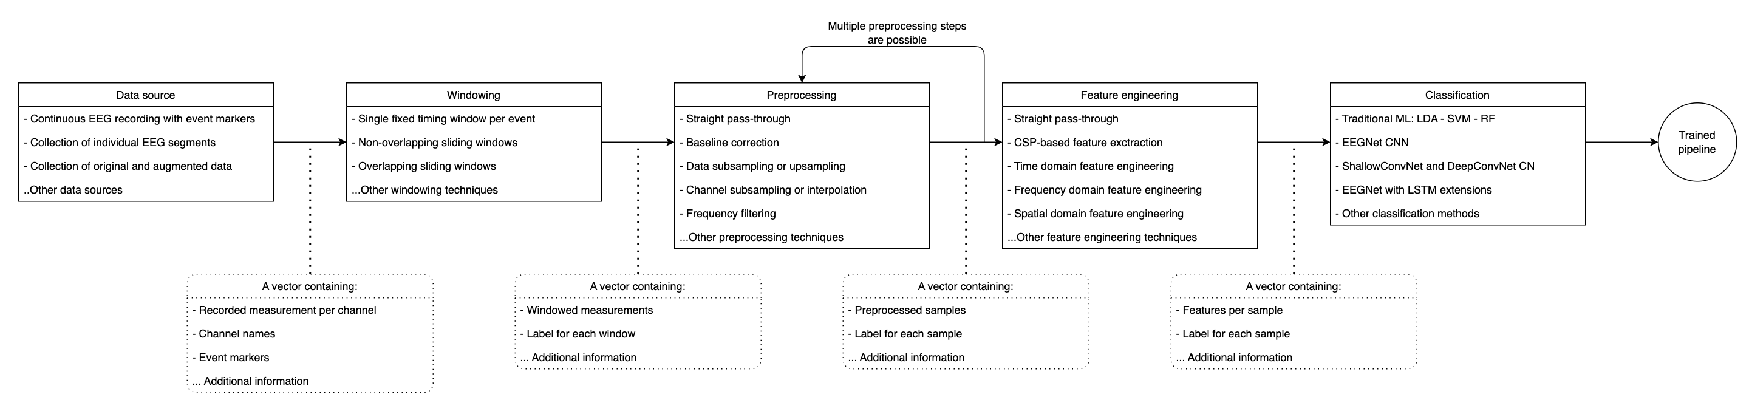
\includegraphics[width=\textwidth]{../images/pipeline/brain_signal_pipeline_training.pdf}
        \captionsetup{width=0.9\linewidth}
        \captionsetup{justification=centering}
        \caption{Components of general training pipeline for brain signal classification annotated with common examples per component.}
        \label{fig:processing_signals_pipeline_ml}
    \end{subfigure}
    \hfill
    \begin{subfigure}{\textwidth}
        \centering
        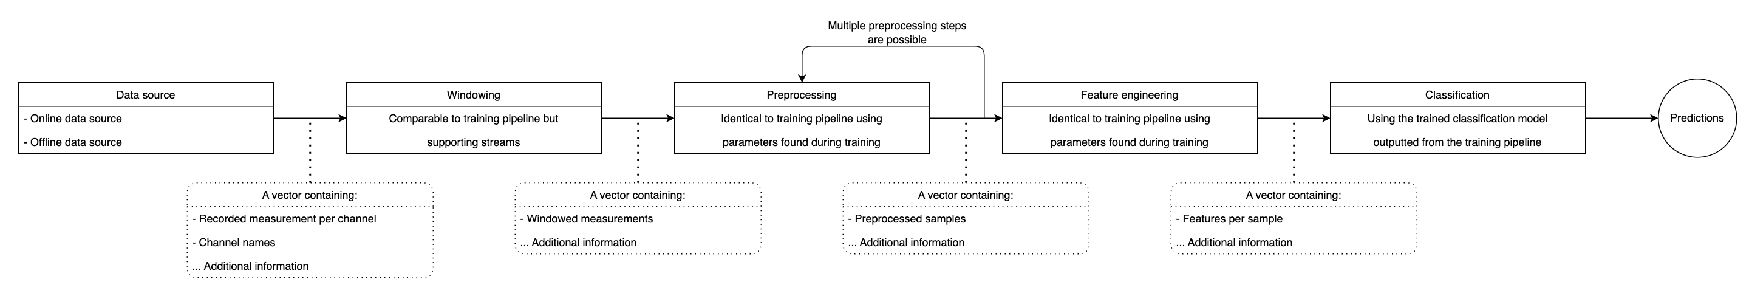
\includegraphics[width=\textwidth]{../images/pipeline/brain_signal_pipeline_predicting.pdf}
        \captionsetup{width=0.9\linewidth}
        \captionsetup{justification=centering}
        \caption{Components of general prediction pipeline for brain signal classification annotated with common examples per component.}
        \label{fig:processing_signals_pipeline_dl}
    \end{subfigure}
    \captionsetup{width=0.9\linewidth}
    \captionsetup{justification=centering}
    \caption{General training pipeline and prediction pipeline used for classifying brain signals.}
    \label{fig:processing_signals_pipeline}
\end{sidewaysfigure}

The general pipeline of classifying brain signals and \gls{eeg}-based \gls{mi} tasks in particular is similar to that of a \gls{cad} systems which was discussed in Section \ref{subsubsec:bci_gaining_popularity_improved_data_processing_better_ml_dl} and shown in Figure \ref{fig:cad_pipeline}.
Whilst the training pipeline and prediction pipeline for classifying brain signals consist of the same components, their input and output are different.
For this reason, this master thesis considers them as two separate pipelines.
The remainder of this section will discuss the components used in these brain signal classification pipelines and the techniques commonly used in each of these components.
Figure \ref{fig:processing_signals_pipeline} provides a visual overview of these pipelines and their components.

% - - - - - - - - - -
% Data acquisition
% - - - - - - - - - -

\subsection{Data source}
\label{subsec:processing_signals_general_pipeline_data_acquisition}

Assuming supervised learning, a \gls{ml} paradigm further discussed in Section \ref{subsec:processing_signals_ml_and_dl_tyes_of_learning_supervision}, input data for the training pipelines should include both the independent variables as wel the dependent variable.
When working with an \gls{eeg} \gls{mi} classification problem, these independent variables are the \gls{eeg} measurements of each channel whilst the dependent variable is the \gls{mi} task performed at a specific time point.
Multiple possibilities exist for providing these variables and the link between them.
Most open-source \gls{mi} \gls{eeg} datasets, such as the one by \citet{eeg_data} used in this master thesis, do this by providing the \gls{eeg} recordings of an entire session as a single 2D matrix (channels x measurement per time point) and the desired labels as an equal width vector containing the marker at any given time point.
The time points are dependent on the sampling frequency and denote the sample number counting from the first sample of the session.
The marker may be the current content of the screen which provides tasks to the user or other event-related information.
Figure \ref{fig:processing_signals_data_source_eeg} combines both the independent and dependent variables into a singular visualisation.

The prediction pipeline only expects the independent variables as its task is to predict the dependent variable.
In theory, these independent variables should be of the same format used during training, but in practice, they might originate from a different source or recording and as such might require additional steps during preprocessing to ensure at least an equal sampling frequency and channel distribution.
This master thesis assumes the device used during training and prediction is identical with equal settings used and as such doesn't require this type of preprocessing.

The prediction pipeline may work in an offline manner, as is the case for the experiments in this master thesis, or in an online manner.
When using offline prediction the data was already recorded and stored before being provided in its totality to the prediction pipeline.
In an online setting, the data is streamed to the prediction pipeline as it is being measured and the prediction pipeline should merge this incoming data to an object that is usable in the next stages itself.
For example, a buffer may be used to collect samples until one second is obtained and pass that to the next step.
In an online setting, windowing is often directly performed on the stream, as discussed next.
Other types of data formatting are possible but they should all provide the same information.

\begin{figure}[ht]
    \centering
    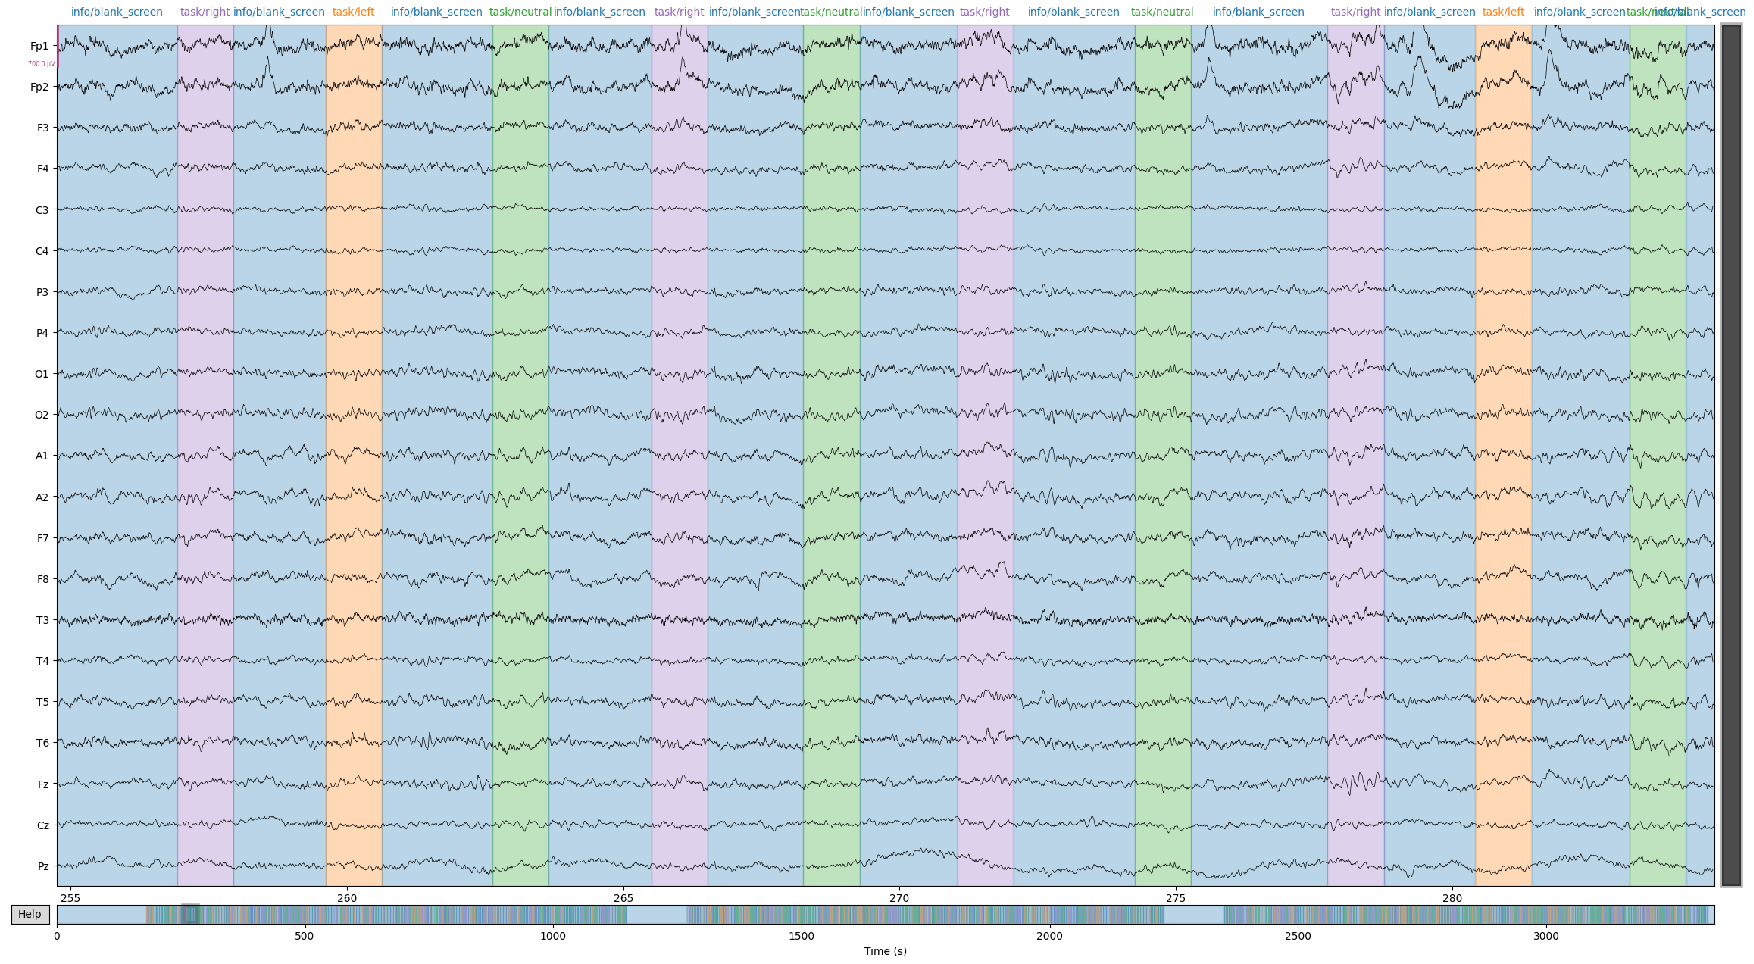
\includegraphics[width=\linewidth]{../images/pipeline/eeg.pdf}
    \captionsetup{width=0.9\linewidth}
    \captionsetup{justification=centering}
    \caption{Visualisation of the \gls{eeg} recording from December 15 2015 overlayed with the provided markers for subject B in the open-source dataset by \citet{eeg_data}. The x-axis depicts the time in seconds, the y-axis depicts which channel of the recording is visualised and the colour overlay represents the active marker.}
    \label{fig:processing_signals_data_source_eeg}
\end{figure}

% - - - - - - - - - -
% Windowing
% - - - - - - - - - -

\subsection{Windowing}
\label{subsec:processing_signals_general_pipeline_windowing}

The data source as described in Section \ref{subsec:processing_signals_general_pipeline_data_acquisition} provides a continous signal over multiple channels.
To process these signals a mechanism has to be in place so that this continuous signal is split into discrete segments.
Such techniques are often referred to as windowing, but the neurophysiological field also refers to it as epoching.
The latter should not be confused with the meaning of epochs in a \gls{ml} setting.
Different types of windowing exist and three common approaches are illustrated in Figure \ref{fig:processing_signals_windowing}.
Using a fixed window surrounding known event points is trivial on the training data and results in the simplest classification task with the most consistent window labels from the three windowing techniques shown in Figure \ref{fig:processing_signals_windowing}.
However, when trying to predict outcomes, the point at which an event occurs has to be known as well.
This information may be known, for example during an offline \gls{mi} classification task or when using a fixed feedback loop in an online manner where actions from the user are accepted at fixed time intervals.

\begin{figure}[ht]
    \centering
    \begin{subfigure}{0.45\textwidth}
        \centering
        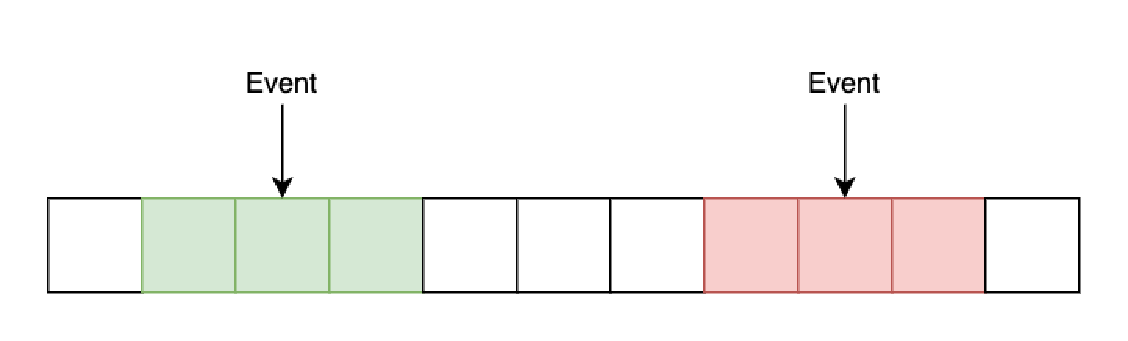
\includegraphics[width=\textwidth]{../images/pipeline/fixed_window.pdf}
        \captionsetup{width=\linewidth}
        \captionsetup{justification=centering}
        \caption{Fixed window surrounding a known event.}
        \label{fig:processing_signals_windowing_non_fixed}
    \end{subfigure}
    \hfill
    \begin{subfigure}{0.45\textwidth}
        \centering
        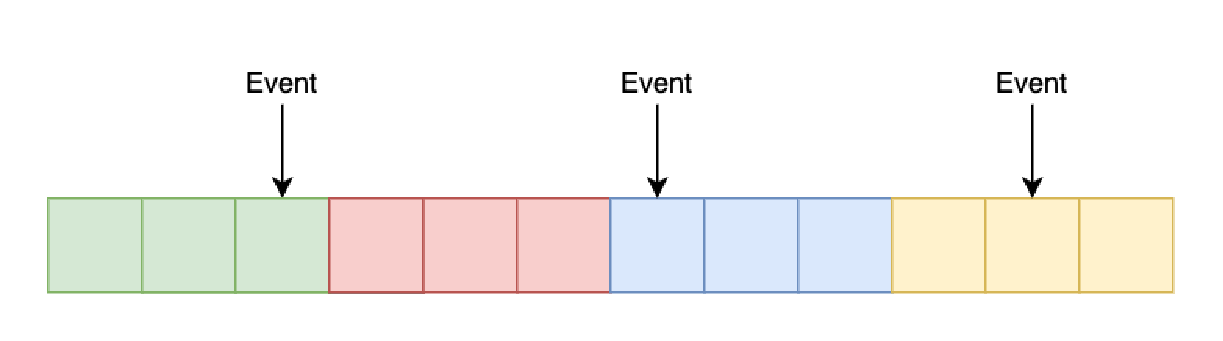
\includegraphics[width=\textwidth]{../images/pipeline/non_overlapping_window.pdf}
        \captionsetup{width=\linewidth}
        \captionsetup{justification=centering}
        \caption{Non-overlapping sliding windows.}
        \label{fig:processing_signals_windowing_non_overlapping}
    \end{subfigure}
    \hfill
    \begin{subfigure}{0.45\textwidth}
        \centering
        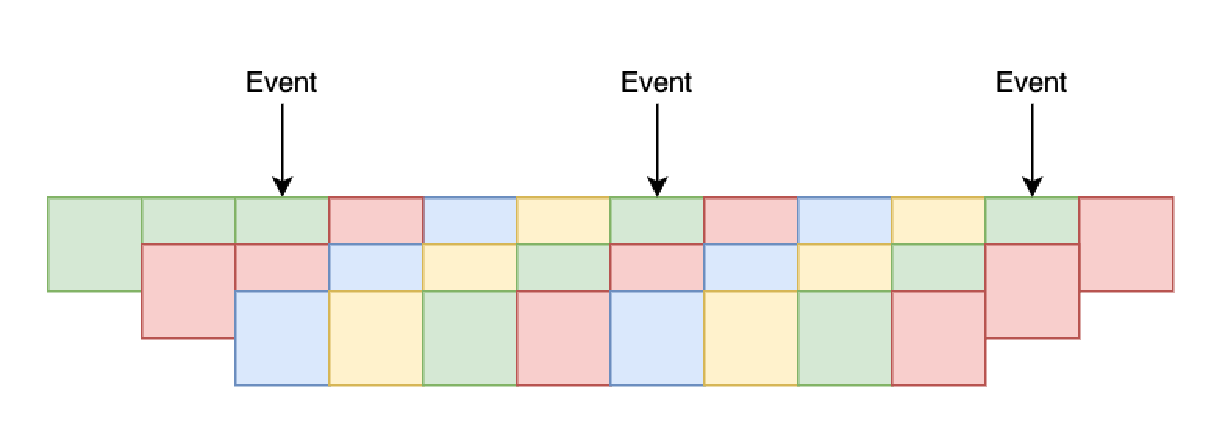
\includegraphics[width=\textwidth]{../images/pipeline/overlapping_window.pdf}
        \captionsetup{width=\linewidth}
        \captionsetup{justification=centering}
        \caption{Overlapping sliding windows}
        \label{fig:processing_signals_windowing_overlapping}
    \end{subfigure}
    \captionsetup{width=\linewidth}
    \captionsetup{justification=centering}
    \caption{Different types of windowing techniques.}
    \label{fig:processing_signals_windowing}
\end{figure}

A more intuitive but computationally harder windowing technique is using sliding windows.
A non-overlapping sliding window technique is shown in Figure \ref{fig:processing_signals_windowing_non_overlapping} and an overlapping technique is shown in Figure \ref{fig:processing_signals_windowing_overlapping}.
Both are trivial to apply to the independent variables but deciding which dependent variable should be related becomes a difficult task.
How much activity from the event should be included for the training window to be considered a sample of that event?
What happens when a window includes two distinct events?
These are questions that should be answered within the context of the application.
When using sliding windows, singular labels such as "task right" may be split into "task right start", "task right hold" and "task right end".

Many different windowing techniques exist that use far more complex strategies than the ones illustrated in Figure \ref{fig:processing_signals_windowing}, especially for controlling the boundaries of the window.
\citet{complex_windowing} discuss some of these more complex windowing techniques in more detail.
When done right, certain sliding window techniques can improve the performance of a \gls{mi} \gls{eeg} classification pipeline compared to even fixed windowing surround a known event, as shown by \citet{sliding_windows_better}.
However, starting a new sliding window at each time point may cause significant computational overhead, increasing both training and prediction time.
The latter can make the prediction pipeline too complex to be run on affordable, low-energy and portable computational hardware as desired by a \gls{bci} system doing local processing.
This master thesis will consider a fixed window of 0.5 seconds and 1.5 seconds surround a known event for both training and prediction.

% - - - - - - - - - -
% Preprocessing
% - - - - - - - - - -

\subsection{Preprocessing}
\label{subsec:processing_signals_general_pipeline_preprocessing}

Brain signals are non-linear as well as non-stationary signals and exact execution of the performed \gls{mi} tasks are bound to differ per subject as already discussed in section \ref{subsec:biomedical_signals_working_with_eeg_generalisation}.
Combining these properties with the poor \gls{snr} of \gls{eeg}, as discussed in Section \ref{tab:biomedical_signals_modalities}, means that raw \gls{eeg} measurements are hard to intepret, even by machines.
Luckily, as discussed by \citet{bci_review_arnau}, a \gls{dl} approach making use of sufficient layer, nodes and training should be capable of learning any mapping from input to output, including any manual preprocessing that can be done.
As such, \gls{dl} approaches can often work directly on this raw \gls{eeg} signal and raw signals in general.
This is one of the most promising aspects of \gls{dl} in multiple fields and it is the reason the one-step \gls{dl} approaches from this master thesis will use no preprocessing besides the \gls{ac} artefact removal that was already performed by the suppliers of the open-source database \citep{eeg_data}.
Traditional two-step \gls{ml} approaches do not have this property of being able to learn any mapping from input to output and as such require at least minimal preprocessing of the data to obtain usable results.
For this reason, many libraries providing the most basic \gls{eeg} preprocessing steps have been developed with MNE by \citet{mne} being the most popular for Python and used in this master thesis.
Some automated pipelines specifically for \gls{eeg} preprocessing have also been proposed, such as the PREP pipeline by \citet{prep_pipeline}. 

% | | | | | | | | | | | | |

\subsubsection{Frequency filtering}
\label{subsubsec:processing_signals_general_pipeline_preprocessing_filter}

One of the most common preprocessing operations done to \gls{eeg} signals is frequency filtering.
Frequency filters come in four main categories: low-pass filters, high-pass filters, band-pass filters and band-stop filters.
The working of these filters in the frequency domain is shown in Figure \ref{fig:processing_signals_filters}.
Again, many variants on how to exactly perform the filter exist.
Some use a harsh filter with no transition band whilst others use a transition band as visualised in Figure \ref{fig:processing_signals_filters}.
As further discussed by \citet{fir_iir_filter}, a first distinction is made between \gls{fir} and \gls{iir} filters.
Most common filter operations are using a band-stop filter to cancel out the \gls{ac} artefacts discussed in Section \ref{subsec:biomedical_signals_working_with_eeg_artefacts} and to filter out frequencies not of interest for the application.
Since these operations are so common they are often included directly in \gls{eeg} equipment with a hardware filter.
This master thesis uses a \gls{fir} filter design using the Blackman window method in some of its experiments to band-pass filter the signal to only include the \gls{mi} frequencies as discussed in Section \ref{subsec:biomedical_signals_working_with_eeg_brain_waves}.
Further details of this exact filter are not of interest for this master thesis and the MNE library supplied functionality is used to obtain the desired filter \citep{mne}.


\begin{figure}[t]
    \centering
    \begin{subfigure}{0.45\textwidth}
        \centering
        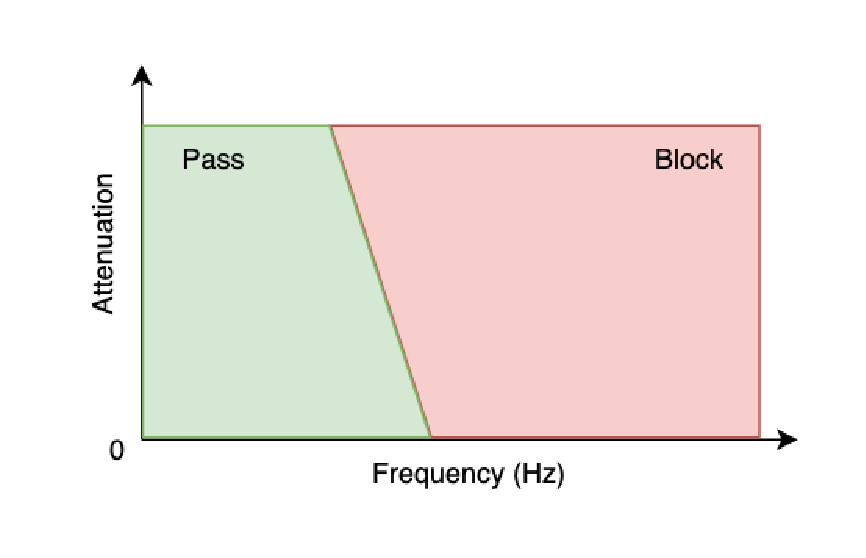
\includegraphics[width=\textwidth]{../images/pipeline/lowpass_filter.pdf}
        \captionsetup{width=\linewidth}
        \captionsetup{justification=centering}
        \caption{Low-pass filter.}
        \label{fig:processing_signals_filters_lowpass}
    \end{subfigure}
    \hfill
    \begin{subfigure}{0.45\textwidth}
        \centering
        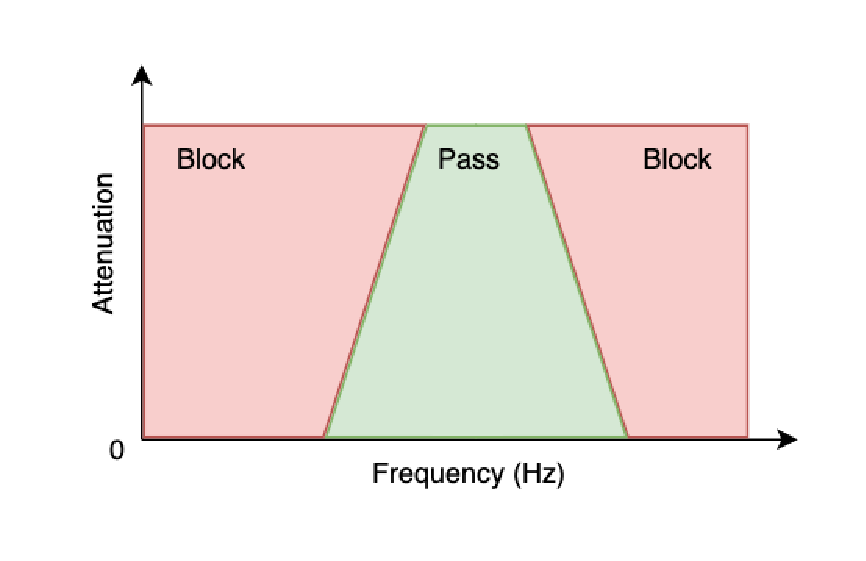
\includegraphics[width=\textwidth]{../images/pipeline/bandpass_filter.pdf}
        \captionsetup{width=\linewidth}
        \captionsetup{justification=centering}
        \caption{Band-pass filter.}
        \label{fig:processing_signals_filters_bandpass}
    \end{subfigure}
    \hfill
    \begin{subfigure}{0.45\textwidth}
        \centering
        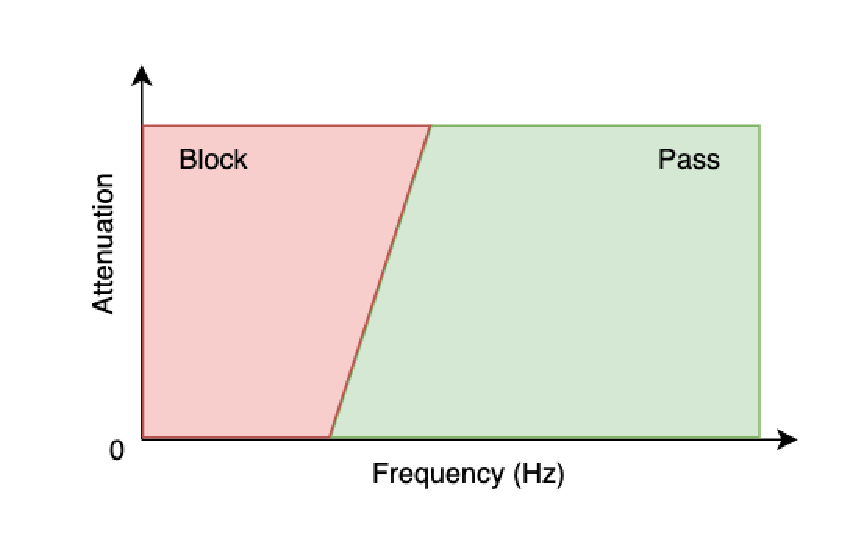
\includegraphics[width=\textwidth]{../images/pipeline/highpass_filter.pdf}
        \captionsetup{width=\linewidth}
        \captionsetup{justification=centering}
        \caption{High-pass filter.}
        \label{fig:processing_signals_filters_highpass}
    \end{subfigure}
    \hfill
    \begin{subfigure}{0.45\textwidth}
        \centering
        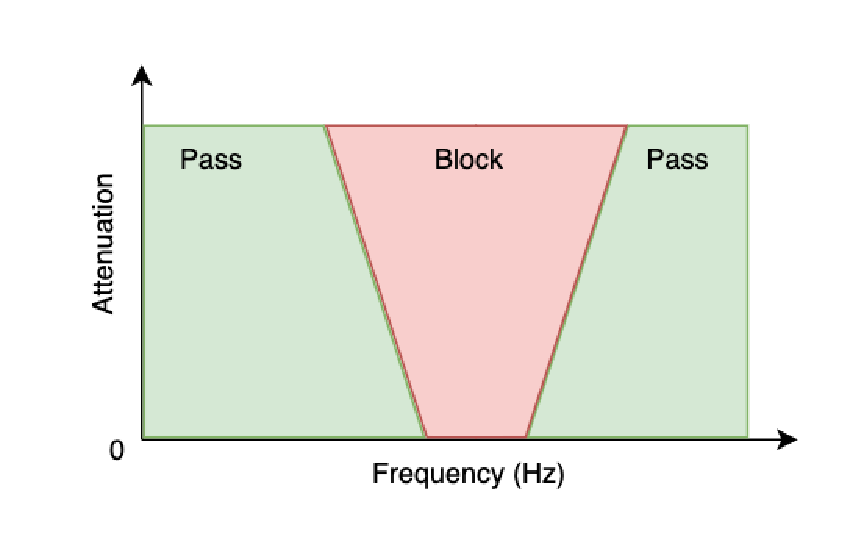
\includegraphics[width=\textwidth]{../images/pipeline/bandstop_filter.pdf}
        \captionsetup{width=\linewidth}
        \captionsetup{justification=centering}
        \caption{Band-stop filter.}
        \label{fig:processing_signals_filters_bandstop}
    \end{subfigure}
    \captionsetup{width=\linewidth}
    \captionsetup{justification=centering}
    \caption{Different types of filtering techniques.}
    \label{fig:processing_signals_filters}
\end{figure}

% | | | | | | | | | | | | |

\subsubsection{Baseline correction}
\label{subsubsec:processing_signals_general_pipeline_preprocessing_baseline_correction}

Another common preprocessing operation is baseline correction on a window.
Baseline correction consists of taking a baseline period and determining the mean voltage of each electrode's measurements during that baseline.
This baseline is most often one or more seconds before an event occurs.
This mean voltage is then subtracted from the remaining signal of each respective channel.
Doing this normalizes each window such that it has a centre closer to zero.
This can help in reducing the non-stationary problem and is used for the traditional two-step \gls{ml} experiments in this master thesis with a baseline period of one second before the event.

% | | | | | | | | | | | | |

\subsubsection{Channel and data downsampling or upsampling}
\label{subsubsec:processing_signals_general_pipeline_preprocessing_subsampling}

Another type of preprocessing is channel subsampling and augmentation through interpolation.
This consists of removing channels not of interest as discussed in Section \ref{subsec:biomedical_signals_working_with_eeg_anatomy} or adding augmented channels by clever interpolation or other approaches from the existing channels.
When a certain channel is known to be bad or artefacts described in Section \ref{subsec:biomedical_signals_working_with_eeg_artefacts} are detected, it may be replaced by an augmented channel during the artefact period as a way of resolving the artefact.
Likewise, if the sampling frequency of \gls{eeg} equipment is too high or low, data subsampling or upsampling may be performed.

% | | | | | | | | | | | | |

\subsubsection{Other preprocessing techniques and preprocessing ordering}
\label{subsubsec:processing_signals_general_pipeline_preprocessing_orders}

There exist many other preprocessing techniques for signals and \gls{mi} \gls{eeg} signals in particular but these fall outside the scope of this master thesis.
Preprocessing can happen in other places of the pipeline than the one shown in Figure \ref{fig:processing_signals_pipeline}, for example, channel subsampling reduces dimensionality and is thus often done as soon as possible to limit unneeded computational overhead.
It is important to note that multiple preprocessing steps may be performed in sequence.
This means that the output of a previous preprocessing step is used in the next and as such the ordering of preprocessing steps can be important depending on the techniques used in the sequence.
It is also important to note that certain preprocessing techniques which learn parameters from the training data should use the same parameters for the prediction pipeline, as redetermining them on the prediction data may alter the data in a way unknown by the already trained classifier later in the pipeline.
Whilst often not the case for preprocessing techniques, this is a subtility of great importance in feature engineering, the next step in the pipeline.



% - - - - - - - - - -
% Feature
% - - - - - - - - - -

\subsection{Feature engineering}
\label{subsec:processing_signals_general_pipeline_features}

Feature engineering, or feature extraction, is the process of representing raw or preprocessed data by numerical features that carry information from the original data related to the problem.
The goal of feature extraction is to simplify a complex data structure by representing it as one or many features that are easier to interpret and/or learn.
This step is crucial in traditional two-step \gls{ml} classification approaches as even the preprocessed data is often too complex for traditional \gls{ml} classifiers to directly learn from.
This differs from preprocessing which aimed to improve the raw data quality, although for some of the discussed preprocessing techniques it could be debated that they are also a type of feature extraction.
As already addressed in Section \ref{subsec:processing_signals_general_pipeline_preprocessing}, some features rely on learned parameters, such as the $\mathbf{W}$ matrix for spatial filters discussed later in this section, these learned parameters should be reused in the prediction pipeline and not redetermined on the prediction data, as this will confuse the classification model and produce unwanted behaviour.

A simple but poor feature extraction technique for \gls{eeg} data would be representing the channels' measurements not by their raw data but by their minimum, maximum, median, first quartile and third quartile, much like a boxplot would.
Whilst this would be easy to interpret, it would carry too little information for a classifier to effectively learn anything but the simplest problems.
Finding appropriate feature extraction techniques is a hard task which has taken years of refinement and has ongoing refinement in many fields, including \gls{eeg} classification and other medical imaging fields \citep{CAD_ml_dl_kbs}.
\gls{eeg} feature extraction methods can be categorized by the domain they work in, namely the time domain, frequency domain, time-frequency domain or spatial domain.
The experiments in this master thesis will only consider \gls{csp} for feature extraction in the traditional \gls{ml} classification approaches, a spatial filtering technique closely related to \gls{pca} used for mainly spatial domain feature extraction.
As discussed in Section \ref{subsec:bci_gaining_popularity_improved_data_processing}, \gls{csp} derived features are commonly used in traditional two-step \gls{ml} classification and the \gls{csp} technique has seen many extensions over the years.
\gls{csp} is further discussed together with its extensions in Section \ref{sec:offline_bci_system_two_step_ml}.

The remainder of this section briefly discusses the feature extraction possibilities in each domain but a more detailed explanation falls outside the scope of this master thesis.
The reader is reffered to chapter 7 of the \gls{bci} book by \citet{bci_book} for an in-depth overview of many feature extraction techniques for \gls{bci} applications in far greater detail.
\Citet{eeg_features} compares the performance of multiple feature extraction techniques for epileptic seizure detection using \gls{eeg}.
\Citet{time_domain_eeg_features} compares multiple feature extraction methods for \gls{eeg}-based \gls{bci} applications in the time domain whilst \citet{timefreq_domain_eeg_features} does the same for feature extraction methods in the frequency and time-frequency domain.


% | | | | | | | | | | | | |

\subsubsection{Time domain feature extraction}
\label{subsubsec:processing_signals_general_pipeline_features_timedomain}

Temporal feature extraction methods work in the time domain, where the \gls{eeg} data is analysed as a time series of voltage measurements per channel.
This is most likely the representation of the data as it comes from the previous preprocessing step in the pipeline and as such doesn't require an additional transformation.
\Citet{time_domain_eeg_features} describes some relatively simple feature extraction methods in the time domain, namely the windows's \gls{mav} per electrode, the amount of times a \gls{zc} and \gls{ssc} occurs per channel and the cumulative \gls{wl}.
When all four of these relatively simple features are combined, surprisingly good accuracies are obtained through intrasession testing \citep{time_domain_eeg_features}.

Many more time domain feature extraction techniques exist and some more examples are given by \citet{eeg_features}.
\citet{eeg_features} discusses some other simple features, including those used by \citet{time_domain_eeg_features}.
For example, the \gls{wl} feature described by \citet{time_domain_eeg_features} is called \textit{total line length} by \citet{eeg_features} and provided in Equation \ref{eq:processing_signals_line_length}.
\Citet{eeg_features} also details more complex features based on the entropy of the signal such as \gls{pe}, \gls{apen}, \gls{fuzzen} and more.

\begin{equation}
    \label{eq:processing_signals_line_length}
    L(X) = \sum_{i=1}^{N-1} |X[i] - X[i - 1]|
\end{equation}


% | | | | | | | | | | | | |

\subsubsection{Frequency domain feature extraction}
\label{subsubsec:processing_signals_general_pipeline_features_freqdomain}

As the name suggests, frequency domain feature extraction happens in the frequency domain.
The frequency domain represents the measured \gls{eeg} signals in terms of frequency rather than time as was the case for the time domain.
To extract features in the frequency domain, the signal represented in the time domain must first be transformed to its frequency domain representation.
The most common way of going from the time domain to the frequency domain is through the use of a \gls{ft} \citep{fourier_transform}.
A  \gls{ft} has the nice property that it can be converted back to the time domain by using the \gls{ift}.
The theoretical \gls{ft} and \gls{ift} make use of integrals from $-\inf$ to $\inf$ and as such can't be directly used on real data.
Many methods have been proposed to estimate this full integral solution, with the \gls{dft} and \gls{idft} being the most common.
The \gls{dft} and \gls{idft} equations are given in Equation \ref{eq:processing_signals_dft} and \ref{eq:processing_signals_idft} respectively.
The output of the \gls{dft} ($X_k$) is a complex number that represents the amplitude and phase of a sinusoidal wave, representing the signal in the frequency domain.
The frequency of this sinusoidal wave is $\frac{k}{N}$ derived from Euler's formula.
\Citet{fast_fourier_explained} discusses the \gls{ft}, \gls{ift}, \gls{dft} and \gls{idft} in more detail.
\Citet{fast_fourier_explained} also discusses that the computation of \gls{dft} can be too complex for many applications and introduces the \gls{fft}, a faster variant of \gls{dft}.
\Gls{fft} is the algorithm that is most commonly used for effective conversion between the time and frequency domain in computer applications.

\begin{equation}
    \label{eq:processing_signals_dft}
    X_k = \sum_{n=O}^{N-1} x_n e^{\frac{-2 \pi i k n}{N}}
\end{equation}

\begin{equation}
    \label{eq:processing_signals_idft}
    x_n = \frac{1}{N} \sum_{k=O}^{N-1} X_k e^{\frac{2 \pi i k n}{N}}
\end{equation}

Once the signal is represented in the frequency domain, most of the frequency domain features are extracted from the \gls{psd}.
The \gls{psd} is a visualisation of the power levels of the frequency component present in the signal.
Figure \ref{fig:processing_signals_psd} show the \gls{psd} of the \gls{eeg} signals previously shown in  Figure \ref{fig:processing_signals_data_source_eeg}.
Note the sharp trough present at 50\gls{hz} due to the \gls{ac} artefact removal that is done by a band-stop filter at that frequency.
As discussed further by \citet{eeg_features}, the features extracted from the \gls{psd} include the energy, \gls{iwmf} and \gls{iwbw} among others.

\begin{figure}[t]
    \centering
    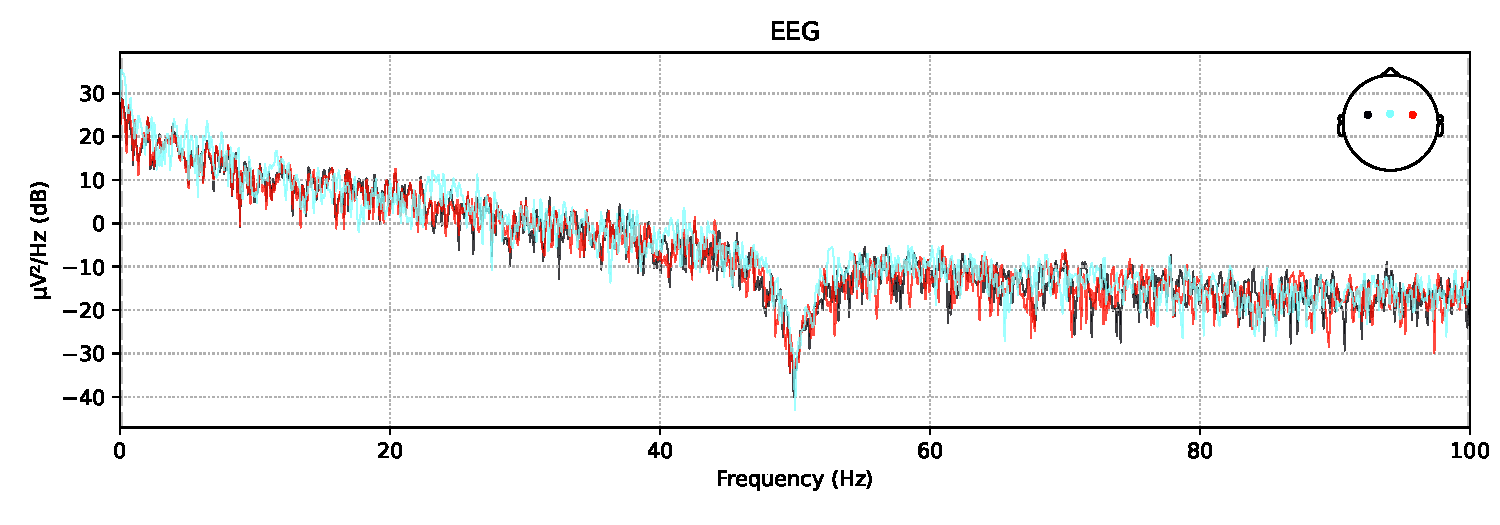
\includegraphics[width=\linewidth]{../images/pipeline/psd.pdf}
    \captionsetup{width=0.9\linewidth}
    \captionsetup{justification=centering}
    \caption{\Glsfirst{psd} for the \gls{eeg} signal previously shown in Figure \ref{fig:processing_signals_data_source_eeg}. Only the C3, Cz and C4 channels are shown.}
    \label{fig:processing_signals_psd}
\end{figure}

% | | | | | | | | | | | | |

\subsubsection{Time-frequency domain feature extraction}
\label{subsubsec:processing_signals_general_pipeline_features_timefreqdomain}

Whilst it is possible to extract features from both the time and frequency domain and rely on the classifier to learn a mapping between them, attempts have been made at combining both domains.
For example, when further windowing the time domain signal into short time segments and using a \gls{ft} on those shorter time segments, a \gls{stft} is obtained.
\Gls{stft} assumes that those shorter time segments are stationary, even if the complete signal from which those time segments are taken was non-stationary.
This allows for using frequency-domain feature extraction on those shorter \gls{ft} signals.
This will result in features that represent frequency domain characteristics but are ordered in a time respective order.
These features could then be seen as individual data points in the time domain and thus can be further processed with time-domain feature extraction techniques.

However, the use of \gls{stft} in \gls{eeg} applications is limited as finding a balance between long enough time segments such that the \gls{ft} is meaningful but short enough so that enough time domain information is retained has been proven challenging.
A better alternative is using \gls{wt}, a technique that has been proven powerful in image compression and many other fields \citep{wavelet_transform_uses}.
Compared to the \gls{ft} that works with sinusoidal waves, \gls{wt} works with wavelets.
These wavelets are characterised by their scale and location.
The scale relates to the frequency domain whilst the location relates to the time domain, showing a clear link with the time-frequency domain.
Compared to \gls{stft}, \gls{wt} does not make any assumptions about stationarity.
The book by \citet{book_wavelet} discusses \gls{wt} in detail.
The technical details and related feature extraction methods of which fall outside the scope of this master thesis.

% | | | | | | | | | | | | |

\subsubsection{Spatial domain feature extraction}
\label{subsubsec:processing_signals_general_pipeline_features_spatialdomain}

As discussed in Section \ref{subsec:biomedical_signals_measuring_brain_modalities}, \gls{eeg} has a relatively poor spatial resolution.
This would suggest that feature extraction based on the spatial domain is bound to perform poorly as well, bet this is not the case.
Many \gls{bci} systems rely on features extracted from \gls{eeg} signals that were spatially filtered with techniques such as \gls{pca}, \gls{ica} and \gls{csp} \citep{bci_book}.
To understand spatial filters, it should be repeated that \gls{eeg} channels don't represent the value of a singular electrode but rather the output of applying a differential amplifier on two channels, as was discussed in Section \ref{subsec:biomedical_signals_measuring_brain_modalities}.
If all these channels have one electrode in common, an alternative set of channels can be created by weighing and combining the original channels \citep{bci_book}.
This is the main idea behind spatial filtering and can be mathematically represented as the matrix equation shown in Equation \ref{eq:processing_signals_spatial_filter}.
In this equation, $\mathbf{X}$ represents the 2D matrix of $N$ channels and $P$ samples.
$\mathbf{W}$ represents the weight matrix with $M$ spatial filters and $N$ channel weights.
Finally, $\mathbf{Y}$ represents the alternative set of channels with $M$ spatially filtered channels and $P$ samples.

There are both data-independent and data-dependent techniques for determining the weight matrix $\mathbf{W}$ of Equation \ref{eq:processing_signals_spatial_filter}.
In some regards, the average reference montage shown in Figure \ref{fig:biomedical_signals_eeg_montages} can be considered a data-independent spatial filter, as it uses a fixed, data-independent $\mathbf{W}$ matrix, namely one that averages all channels.
A more complex but comparable data-independent spatial filter is using one of many variants of surface Laplacian spatial filtering.
Intuitively, these types of Laplacian filters use only the electrodes at a certain spatial distance for determining the average.
Simple variants may consider each electrode in the region of interest equally important whilst others might use a weighted average based on the spatial distance of the electrode.
Surface Laplacian spatial filtering has proven successful in improving the source localisation capabilities of \gls{eeg} by filtering out the signals present in multiple electrodes and keeping only those unique to the electrode of interest \citep{improve_eeg_spatial_laplacian1, improve_eeg_spatial_laplacian2, improve_eeg_spatial_laplacian3}.


\begin{equation}
    \label{eq:processing_signals_spatial_filter}
    \begin{bmatrix} 
        y_{11} & y_{12} & \dots \\
        \vdots & \ddots & \\
        y_{M1} &        & y_{MP} 
    \end{bmatrix} = 
    \begin{bmatrix} 
        w_{11} & w_{12} & \dots \\
        \vdots & \ddots & \\
        w_{M1} &        & w_{MN} 
    \end{bmatrix}
    \begin{bmatrix} 
        x_{11} & x_{12} & \dots \\
        \vdots & \ddots & \\
        x_{N1} &        & x_{NP} 
    \end{bmatrix}
\end{equation}


However, by far the most commonly used spatial domain feature extraction happens on data after a data-dependent spatial filter such as \gls{pca}, \gls{ica} or \gls{csp} has been applied.
These data-dependent spatial filters optimize the $\mathbf{W}$ matrix from Equation \ref{eq:processing_signals_spatial_filter} based on measured \gls{eeg} signals.
\Gls{pca} creates a $\mathbf{W}$ matrix such that the resulting signal has the highest proportion of amplitude variance from the original signals matrix $\mathbf{X}$ \citep{bci_book}.
Whilst this can be successful, \gls{pca} only uses the values from the independent variables for creating the $\mathbf{W}$ matrix and as such the created matrix is not optimized for best discrimination of the dependent variable.
Imagine for example a $\mathbf{X}$ matrix that was not preprocessed to remove the \gls{ac} artefacts described in Section \ref{subsec:biomedical_signals_working_with_eeg_artefacts}.
Since this line current noise is so present, \gls{pca} will consider it as one of the most important \gls{pca} components even though it carries no information for the problem.
\Gls{ica} could be seen as a variant of \gls{pca} that wishes to create a $\mathbf{W}$ matrix such that the resulting signal consists of independent channels.
However, as described by \citet{bci_book}, using \gls{ica} forms multiple challenges in \gls{bci} applications due to its computational cost and often imperative way of determining the number of independent channels to be found.
Besides this, \gls{ica} also only rely on the independent variable and as such is not further considered for this master thesis.

\Gls{csp} is a type of spatial filtering closely related to \gls{pca} that does use the dependent variable to create a set of new channels that are optimized to solve the problem.
This makes \gls{csp} incredibly powerful and studied in \gls{bci} research, as already addressed in Section \ref{subsec:bci_gaining_popularity_improved_data_processing}.
\Gls{csp} will be discussed in further detail together with its extensions in Section \ref{sec:offline_bci_system_two_step_ml}.
\Citet{bci_book} provides a more in-depth overview of all three of these spatial filtering techniques.

% | | | | | | | | | | | | |

\subsubsection{The promise and downfall of feature extraction}
\label{subsubsec:processing_signals_general_pipeline_features_dl_link}

Manual feature extraction is done in what this master thesis refers to as traditional two-step \gls{ml}. 
These traditional two-step \gls{ml} approaches have some attractive properties but also some fundamental limitations.
Manual feature extraction such as the one discussed in this section mostly tries to implement human knowledge about a problem as an algorithm.
Features that are derived are those that an expert deems fit for describing and learning the problem.
This is great in terms of explainability and interpretability, as combined with the right \gls{ml} classification algorithm such as \gls{rf} it can give direct insight into how a prediction pipeline came to its conclusion.
This is desired in many fields, especially the medical one.
As such, traditional two-step \gls{ml} still has significant ongoing research as is shown by the many alternatives on \gls{csp} that have been proposed, as further discussed in Section \ref{sec:offline_bci_system_two_step_ml}.

However, as discussed by \citet{CAD_ml_dl_kbs} for medical lung imaging applications, \gls{dl} that learns some form of features from data in an automated manner outperform traditional two-step \gls{ml} classification in many tasks.
This lies in the power of \gls{dl} being able to learn features that might be unknown by experts and thus can't be encoded for manual feature extraction.
Research in disease detection, such as \citet{attia} findings of using a \gls{cnn} to detect \gls{af} from normal sinus rhythm \gls{ecg} has shown just that.
Given the human understanding of the brain is still limited as discussed in Section \ref{subsec:bci_opportunities_obstacles_complex}, it is likely that the right \gls{dl} models will learn features that are far more descriptive of the problem but not yet understood or discovered by experts.
This is also likely the reason that \gls{cnn} based models, such as those by \citet{eeg_model_eegnet} and \citet{eeg_model_hbm}, have matched or even outperformed the capabilities of state-of-the-art traditional two-step \gls{ml} approaches that have taken years of refinement.
The main limiting factor for \gls{dl} is the lack of explainability and interpretability since these approaches are seen as black box approaches.
However, as \ref{subsec:offline_bci_system_one_step_dl_interpreting} will discuss in more detail, attempts have been made at offering some insight into the working of these models.
These attempts at clarifying what a \gls{dl} model learns can provide experts with a deeper understanding of the problem \citep{dl_book}.


% - - - - - - - - - -
% Classification
% - - - - - - - - - -

\subsection{Classification}
\label{subsec:processing_signals_general_pipeline_classification}

The last step of the general pipeline for classifying brain signals is the classification itself.
In the training pipeline, the classification model used will be trained by providing it both the independent variables processed in the previous pipeline steps and the dependent variables.
The goal of the classification model is to learn a mapping from those independent variables to the dependent variable.
As discussed, the independent variable is either the features extracted from preprocessed data in case of traditional two-step \gls{ml} or the minimally preprocessed raw \gls{eeg} signal in case of one-step \gls{dl} approaches.
The dependent variable is the label of the \gls{mi} task that is being performed.
The prediction pipeline uses this trained model to predict the dependent variable based on only the independent variables.

A regression pipeline for processing brain signals would differ in this part, as it would not output the label of \gls{mi} task performed but a continuous value.
Classification and regression are types of supervised learning, the \gls{ml} paradigm assumed by the proposed pipeline.
The difference between regression and classification and why classification is more popular for \gls{bci} applications relying on \gls{mi} \gls{eeg} data is further discussed in Section \ref{subsec:processing_signals_ml_and_dl_tyes_of_learning_supervision}.

Many different classification models exist with the popular traditional \gls{ml} algorithm providing Python library \gls{sklearn} by \citet{sklearn} having over ten different \gls{ml} classifiers each with their own tunable parameters available.
For \gls{dl} classification models, Keras and Tensorflow \citep[Python \gls{dl} libraries by][]{keras, tensorflow} provide tens of layers that all can be combined to create an almost endless amount of unique classification models.
Countless combinations of both these traditional \gls{ml} and \gls{dl} approaches have been tried in \gls{eeg}-based \glspl{bci}.
As such, discussing all these different classification models falls outside the scope of this master thesis.
The interested reader is referred to both the original review paper on classification models for \gls{eeg}-based \glspl{bci} by \citet{eeg_based_bci_classification_models_old} and the updated version \citep{eeg_based_bci_classification_models}.

The traditional two-step \gls{ml} classifiers used in the experiments of this master thesis will be discussed in more detail in section \ref{subsec:processing_signals_ml_and_dl_ml_classifiers}.
In particular, \gls{lda}, \gls{svc} (based on \gls{svm}) and \glsfirst{rf} are discussed.
Likewise, section \ref{subsec:processing_signals_ml_and_dl_dl_classifiers} will discuss the most important concepts of \gls{dl} used for the \gls{dl} experiments in this master thesis.



% ---------------------------------------------- 
% ML AND DL TECHNIQUES
% ---------------------------------------------- 

\section{Machine learning and deep learning for classification}
\label{sec:processing_signals_ml_and_dl}

Machine learning is a broad field in computer science that focuses on algorithms aiming to relate specific data with a task at hand.
Many different \gls{ml} paradigms exist, with this master thesis focusing on supervised learning with classification in particular.
Throughout this master thesis, the terms \textit{traditional two-step \gls{ml}} and \textit{one-step \gls{dl}} were used quite often.
This section will explain how \gls{dl} is a subfield of \gls{ml} and the most important difference between \gls{dl} and \gls{ml} are given.
Three traditional \gls{ml} classifiers are discussed in more detail: \gls{lda}, \gls{svc} and \gls{rf}.
The most important concepts of \gls{dl} for this master thesis will also be discussed, including fully connected layers (as seen in \glspl{ann}), convolutional layers and pooling layers (as seen in \glspl{cnn}) along with various important concepts such as dropout, batch normalization and activation functions.
For even further insights, the interested reader is referred to the \gls{ml} book by \citet{ml_book} and \gls{dl} book by \citet{dl_book} which cover all \gls{ml} and \gls{dl} concepts needed for this master thesis and much more.
The practical book on both traditional two-step \gls{ml} model development using \gls{sklearn} and one-step \gls{dl} model development using Keras and Tensorflow by \citet{ml_dl_book} covers all practical aspects needed to understand the Python implementations of the experiments performed in this master thesis.

% - - - - - - - - - -
% Common regular ML classifiers
% - - - - - - - - - -

\subsection{Machine learning paradigms}
\label{subsec:processing_signals_ml_and_dl_tyes_of_learning_supervision}

% discuss; supervised -> classi en regres maar regres niet common bci mi eeg want te weinig info

% Supervised, Semi-Supervised, Unsupervised, and Self-Supervised Learning

% The most common form of ML is supervised learning, in which we assume that the data is presented as a set of input-output pairs, a dataset, which we call labeled data, as each input is labeled with its corresponding output.

% The most common form of ML is supervised learning, in which we assume that the data is presented as a set of input-output pairs, a dataset, which we call labeled data, as each input is labeled with its corresponding output (Caruana and NiculescuMizil 2006). Alternatively, unsupervised learning techniques do not use outputs for learning, but rather learn the (unknown) structure of the data. Semi-supervised learning methods use both labeled and unlabeled data, usually to learn the structure of the training data to become able to generate more (artificial) training points (Aznan et al 2019), that are used for conventional supervised learning in a second learning phase. Self-supervised learning (Jing and Tian 2019) is a similar approach that is used to learn the relevant structure in EEG data by first learning an unsupervised pretext task, after which the model is further trained on the target task with labeled data (Banville et al 2020, Kostas et al 2021). The remainder of this review will focus on supervised learning methods.

% Semi-supervised learning methods use both labeled and unlabeled data. Their objective is to learn a supervised learning task, even in cases where only a small amount of training data is available. Usually, semi-supervised approaches learn the structure of the training data to become able to generate more (artificial) training points (Aznan et al 2019), that are used for conventional supervised learning in a second learning phase. Self-supervised learning (Jing and Tian 2019) is a similar approach which is currently gaining traction in the larger ML community. This technique was previously used to learn the relevant structure in EEG data by first learning an unsupervised pretext task, after which the model is further trained on the target task with labeled data (Banville et al 2020, Kostaset al 2021). The remainder of this review will focus on supervised learning methods.

% Therefore, low-confidence labelled data is often used in a semi-supervised fashion as explained by \citet{deep_learn_low_label}.

In \gls{ml} four major categories of learning are distinguished: supervised, unsupervised, semi-supervised and reinforcement learning.
The following will briefly discuss the difference between these four major \gls{ml} paradigms.


% | | | | | | | | | | | | |

\subsubsection{Supervised learning}
\label{subsubsec:processing_signals_ml_and_dl_tyes_of_learning_supervision_supervised}

In supervised learning, the dataset used for learning consists of $N$ \textit{labeled samples}: $\{(\textbf{x}_i, y_i)\}^N_{i=1}$.
The feature vector $\textbf{x}_i$ contains the independent variable(s) and $y_i$ contains the label of a specific sample $i$.
The feature vector can contain all sorts of information in all sorts of data structures but the order of elements in the feature vector $\textbf{x}_i$ must be respected for all samples.
For examples, if the second feature of sample $i$ in the feature vector represents the age of a subject $i$ ($\textbf{x}_i^2 = \text{age of subject }i$), it should also represent age for any other subject $j$ ($\textbf{x}_j^2 = \text{age of subject }j$).
The label $y_i$ can also be any data type, although it most belongs to a finite set of classes (e.g. whether an email is considered spam or not expressed as a string or integer) or an infinite set of continuous values (e.g. a decimal denoting the risk of having a disease).

Within supervised learning, a further division can be made between classification and regression.
Classification consists of predicting the class of a sample ($y_i$ is a class) based on its feature vector ($\textbf{x}_i$).
Regression consists of predicting the real-valued label ($y_i$ is a continous value) based on its feature vector ($\textbf{x}_i$).
In both cases, the goal of supervised learning is to find a model that maps the feature vector $\textbf{x}_i$ to the corresponding label $y_i$ as good as possible.

Supervised learning is one of the most commonly studied \gls{ml} paradigms, especially for \gls{eeg}-based \gls{bci} where it is almost exclusively used for classification \citep{bci_review_arnau}.
In the proposed pipeline for \gls{mi} \gls{eeg} data classification from Section \ref{sec:processing_signals_general_pipeline}, the feature vector contains $\textbf{x}_i$ either the features extracted in the feature extraction phase when using two-step \gls{ml} or the minimally preprocessed \gls{eeg} signal when using one-step \gls{dl}.
One sample $i$ corresponds with the data of one window.
The classes possible for $y_i$ are the \gls{mi} tasks that the user is allowed to perform.



% | | | | | | | | | | | | |

\subsubsection{Unsupervised learning}
\label{subsubsec:processing_signals_ml_and_dl_tyes_of_learning_supervision_unsupervised}

In unsupervised learning the dataset only contains the feature vector of samples, it is a collection of unlabeled samples: $\{(\textbf{x}_i)\}^N_{i=1}$.
Multiple goals for unsupervised learning exist, with clustering being the most common.
In clustering, the model is asked to find groupings (clusters) in its data and return the group (cluster) a new sample belongs to.
In a clustering task, the model is expected to find patterns in the data which might reveal interesting outcomes.
Other common unsupervised learning tasks include dimensionality reduction and outlier detection amongst others \citep{ml_book}.
Unsupervised learning is most commonly used in the \gls{bci} field for calibrating an already trained model to a new subject or session without requiring explicit calibration from the user where the user is asked to perform a specific task.
This is a promising technique in the \gls{bci} as it uses the data already collected by a \gls{bci} to further improve itself.
\Citet{unsupervised_learning_bci} reviews and tests this technique in an \gls{erp}-based \gls{bci} setting.


% | | | | | | | | | | | | |

\subsubsection{Semi-supervised learning}
\label{subsubsec:processing_signals_ml_and_dl_tyes_of_learning_supervision_semisupervised}

The above-given example of using unsupervised learning to perform calibration without requiring specific actions from a \gls{bci} user shows that unlabeled data can enhance the quality of what is otherwise a supervised learning problem.
Semi-supervised learning builds on the same idea, both labelled and unlabeled samples are provided for learning what is otherwise a supervised learning goal.
This is especially handy in cases where a large amount of unlabeled data is available but only a small amount of labelled data is present.
Since this is the case for most applications of the \gls{bci} field, this type of learning has seen a growing interest in the field \citep{semi_supervised_bci1, semi_supervised_bci2, semi_supervised_bci3}.
These approaches deliver promising results compared to traditional supervised learning approaches with similar classification results but requiring fewer training samples and thus shorter calibration.
However, more research is needed to ensure the reliability of these methods in learning useful properties from the provided unlabeled data.


% | | | | | | | | | | | | |

\subsubsection{Reinforcement learning}
\label{subsubsec:processing_signals_ml_and_dl_tyes_of_learning_supervision_rl}

\Gls{rl} is a completely different approach to \gls{ml} as those described before.
In \gls{rl} an \textit{agent} ("an algorithm") lives in the real world or a simulation.
The world the agent lives in, albeit simulated or not, is called the environment and the agent can perceive this environment through a feature vector that is called a \textit{state}.
The agent can then perform \textit{actions} in the environment which may change the state.
After a sequence of actions, the agent receives a \textit{reward}, which is comparable to a label and can be dependent on multiple factors including the final state and the time it took to get there.
The goal of the agent is to learn a policy for choosing the best action for each possible state which yields the best reward.
Whilst \gls{rl} is an interesting approach that has yielded algorithms which outperform human experts in multiple games such as Go \citep{alphago}, its usability in the \gls{bci} field is limited as of now and as such this paradigm is not discussed further.


% - - - - - - - - - -
% Difference ML & DL
% - - - - - - - - - -

\subsection{Traditional two-step ML vs one-step DL classifiers}
\label{subsec:processing_signals_ml_and_dl_difference}

Throughout the discussion of the general brain signal classification pipeline in Section \ref{sec:processing_signals_general_pipeline}, it was discussed how \gls{dl} approaches differ from traditional \gls{ml} approaches by being able to learn directly from the raw, or minimally preprocessed, \gls{eeg} signal.
Since \gls{dl} is a subdivision of \gls{ml}, the difference between the two approaches is often emphasized by calling these \gls{ml} classifiers that require explicit feature extraction \textit{tradition two-step \gls{ml}} whilst \gls{dl} approaches who don't require this step are referred to as \textit{one-step \gls{dl}}.

As described by \citet{nn_can_learn_from_raw}, \gls{dl} models are universal function approximaters.
This is the foundational reason why \gls{dl} can learn any preprocessing or feature extraction step from labelled data, given sufficient layer, nodes and training as discussed in Section \ref{subsec:processing_signals_general_pipeline_preprocessing}.
Thus, \gls{dl} models learn some form of feature extraction during training.
As discussed in Section \ref{subsec:processing_signals_general_pipeline_classification} this makes it possible to gain additional knowledge of a problem by interpreting these features created by the \gls{dl} model.
Whilst this is a non-trivial task due to the black-box property of \gls{dl}, it has been achieved for multiple types of \gls{dl} models in multiple fields \citep{eeg_model_hbm, black_box_insight1, black_box_insight2}.
For some of the experiments in this master thesis, the \gls{cnn} based \gls{eeg} classification models DeepConvNet and ShallowConvNet by \citet{eeg_model_hbm} are used. 
For these models, a visualisation of their learned features exists, as further discussed in Section \ref{subsec:offline_bci_system_one_step_dl_interpreting}.

% - - - - - - - - - -
% Common traditional ML classifiers
% - - - - - - - - - -

\subsection{Common traditional two-step ML classifiers}
\label{subsec:processing_signals_ml_and_dl_ml_classifiers}

% To discuss: LDA, SVM and RF
% bekijk ml_strats_used_in_papers

% https://doi.org/10.1145/1143844.1143865 veergelijkt SVM en RF en andere

As discussed in Section \ref{subsec:processing_signals_general_pipeline_classification}, many different tradition two-step \gls{ml} classifiers exist.
The experiments in this master thesis make use of three such classifiers: \gls{lda}, \gls{svc} (based on \gls{svm}) and \gls{rf}.
This section will introduce these \gls{ml} techniques in what follows.
For more theoretical details, the interested reader is referred to the work by \citet{ml_book}.
For more practical implementation details, \citet{ml_dl_book} provides a discussion on how to use these models with \gls{sklearn}, the same Python library used for the experiments in this master thesis \citep{sklearn}.



% | | | | | | | | | | | | |

\subsubsection{Linear Discriminant Analysis (LDA)}
\label{subsubsec:processing_signals_ml_and_dl_ml_classifiers_lda}

As the name suggests, \gls{lda} uses linear decision boundaries to classify data points.
The most attractive feature of \gls{lda} is the fact that it has no hyperparameters to tune.
For this reason, \gls{lda} is often used when already hyperparameter tuning many parameters for the feature extraction components, as eliminating classifier finetuning can speed up to process significantly.
Adding to this, \gls{lda} is inherently multiclass, has an easy-to-compute closed form solution and has been shown to work well with \gls{csp}-based feature extraction \citep{csp_lda1, csp_lda2}.
These are the exact reasons \gls{lda} is used in this master thesis when using complex hyperparameter tuning setups for \gls{csp} and frequency filtering.
However, \gls{lda} assumes that the features from each feature vector $\textbf{x}_i$ have a normal (Gaussian) distribution and thus the data is a multivariate Gaussian.
It also assumes that each feature $\textbf{x}^j_i$ has a comparable variance around their mean on average.
These assumptions are not super strict and as discussed, it has been shown that \gls{lda} works well with \gls{csp}-based feature extraction \citep{csp_lda1, csp_lda2}.

\Gls{lda} was first proposed by \citet{lda_invention} as a dimensionality reduction technique.
It is inspired by \gls{pca} but makes use of both the feature vector $\textbf{x}_i$ and class labels $y_i$, where \gls{pca} only used the feature vector $\textbf{x}_i$.
The dimensionality reduction of \gls{lda} works by maximizing the ratio of the intra-class scatter, given in Equation \ref{eq:processing_signals_lda_intrascatter}, to the inter-class scatter, given in Equation \ref{eq:processing_signals_lda_interscatter} \citep{lda_classification}.
In these equations, $n$ denotes the number of classes, $c_i$ denotes the class $i$, $m_i$ denotes the number of training samples for class $i$, $\mathbf{\bar{x}_i}$ is the mean for class $i$, and $\mathbf{\bar{x}}$ is the total mean vector derived from Equation \ref{eq:processing_signals_lda_total_mean}.
From these values, the linear transformation $\Phi$ can be derived by solving the eigenvalue problem shown in Equation \ref{eq:processing_signals_lda_linear_transform}.
This linear transformation ($\Phi$) can then be used for predicting the class $c_{pred}$ of a new sample $\mathbf{x}_{new}$ in the transformed space by using any arbitrary distance measure $d$ in equation \ref{eq:processing_signals_lda_classificiation}.
\Citet{lda_classification} discusses \gls{lda} classification in further detail.

\begin{equation}
    \label{eq:processing_signals_lda_intrascatter}
    \hat{\Sigma}_w = S_1 + ... + S_n = \sum^n_{i = 1} \sum_{x \in c_i} (\mathbf{x} - \mathbf{\bar{x}_i}) (\mathbf{x} - \mathbf{\bar{x}_i})'
\end{equation}

\begin{equation}
    \label{eq:processing_signals_lda_interscatter}
    \hat{\Sigma}_b = \sum^n_{i = 1} m_i (\mathbf{\bar{x}_i} - \mathbf{\bar{x}}) (\mathbf{\bar{x}_i} - \mathbf{\bar{x}})'
\end{equation}

\begin{equation}
    \label{eq:processing_signals_lda_total_mean}
    \mathbf{\bar{x}} = \frac{1}{m} \sum^n_{i = 1} m_i \mathbf{\bar{x}_i}
\end{equation}

\begin{equation}
    \label{eq:processing_signals_lda_linear_transform}
    \hat{\Sigma}_b \Phi = \lambda \hat{\Sigma}_w \Phi
\end{equation}

\begin{equation}
    \label{eq:processing_signals_lda_classificiation}
    c_{pred} = \underset{j}{\arg\min} d(\mathbf{x}_{new} \Phi, \mathbf{\bar{x}}_j \Phi)
\end{equation}

% | | | | | | | | | | | | |

\subsubsection{Support vector machines (SVM)}
\label{subsubsec:processing_signals_ml_and_dl_ml_classifiers_svm}

\Gls{svm} are a popular supervised \gls{ml} algorithm for classification (\gls{svc}), regression, outlier detection and more \citep{svm_explained}.
The fundamental idea behind \gls{svm} was first introduced by \citet{first_svm} but has since seen some changes to become the algorithm it is known as today \citep{svm_history}.
The general ideas of using \gls{svm} as a classifier will be discussed here.
For a more detailed explanation or more information about the use of \gls{svm} for regression and other tasks, the reader is referred to the work by \citet{svm_explained}.

Just like \gls{lda}, \gls{svm} also uses linear decision boundries, however, it is not inherently multiclass like \gls{lda}.
multiclass classification using \gls{svm} can be established using a wide variety of methods, such as a one-vs-rest scheme or a one-vs-one scheme.
The \gls{sklearn} implementation of the \gls{svm} classifier, \gls{svc}, uses a one-vs-one scheme \citep{sklearn}.
This means that multiple \gls{svm} are made, one for each possible pair of classes, and the prediction of a new sample is made based on a (potentially weighted) majority vote.

There are three important concepts to address about \gls{svm} classifier: linear boundary optimisation, soft margins and the kernel trick.
When a problem is linearly separable there exists not one but many linear decision boundaries, as is shown in Figure \ref{fig:processing_signals_svm_boundary_multiple}.
Whilst intuitively one decision boundary shown in Figure \ref{fig:processing_signals_svm_boundary_multiple} might be better than another, they all separate the training data equally well and without making any assumptions, no \textit{best} decision boundary can be chosen.

\begin{figure}[t]
    \centering
    \begin{subfigure}{0.45\textwidth}
        \centering
        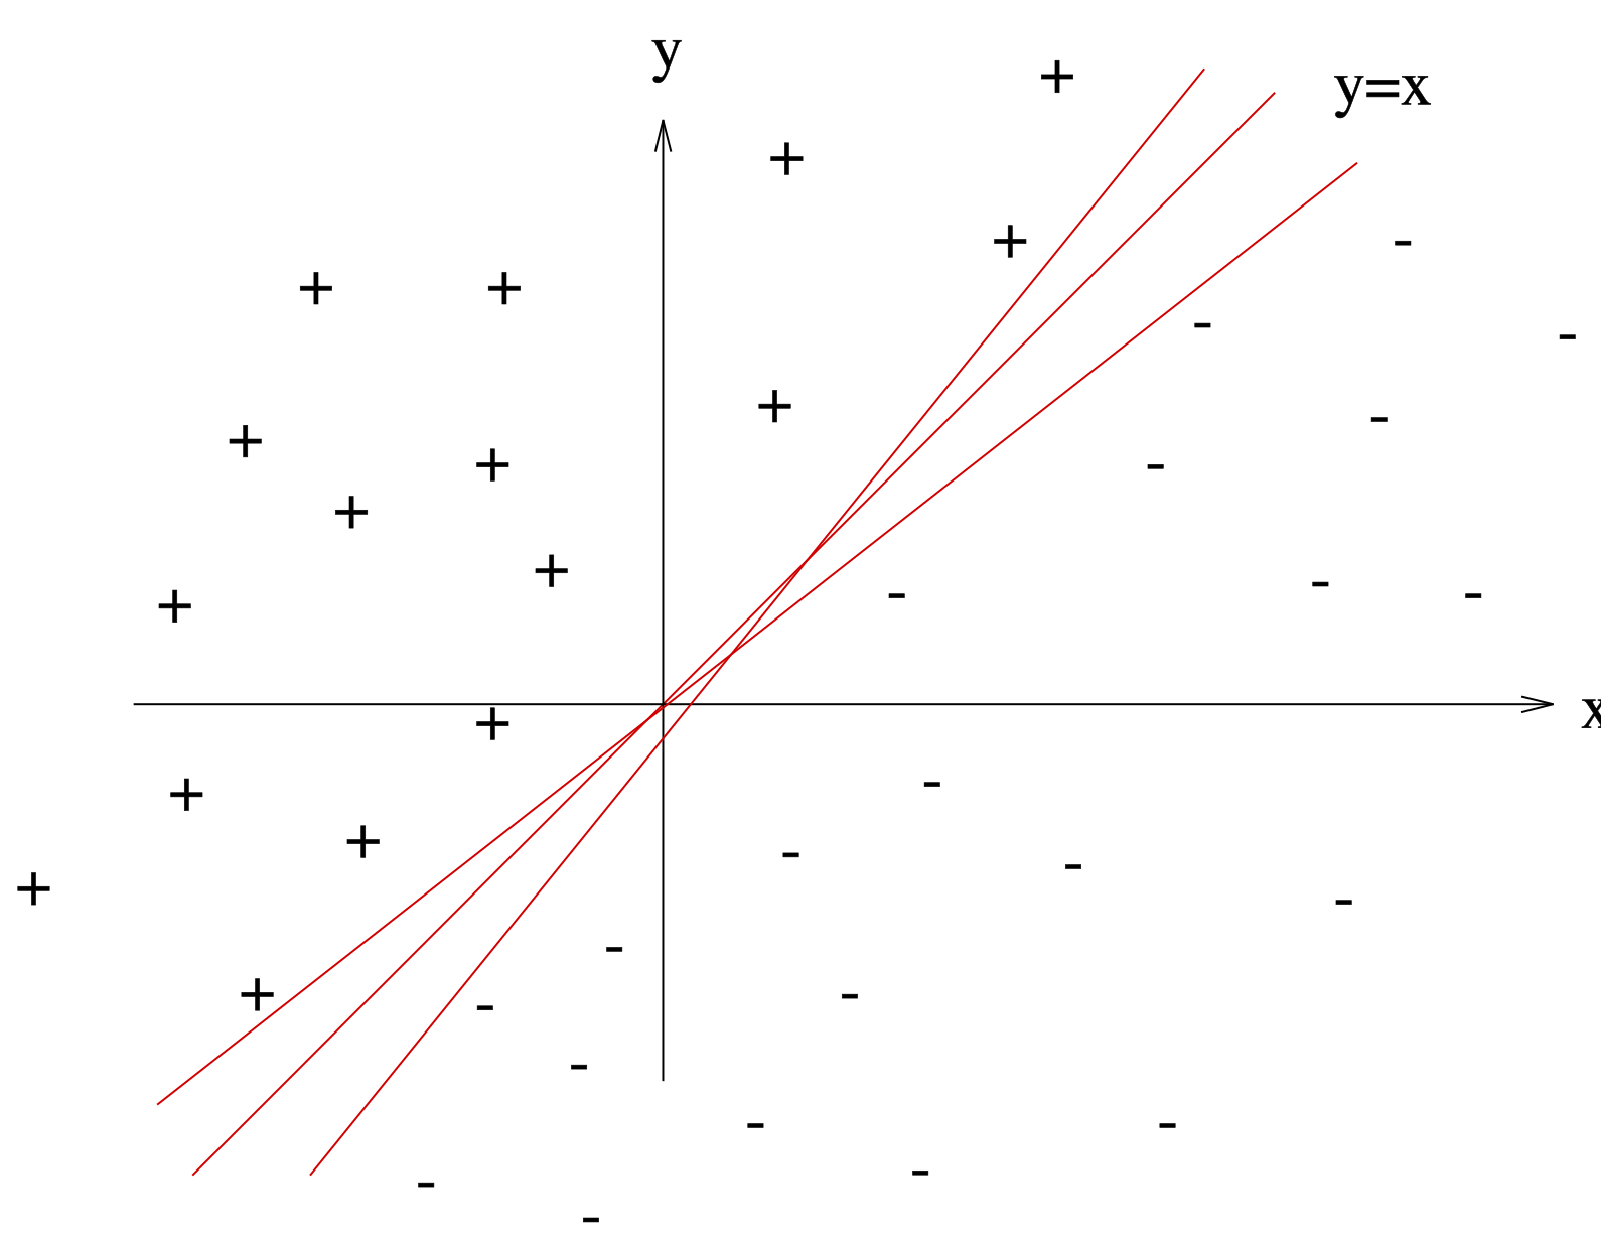
\includegraphics[width=\textwidth]{../images/pipeline/svm_multiple_boundaries.pdf}
        \captionsetup{width=\linewidth}
        \captionsetup{justification=centering}
        \caption{Multiple equally good linear decision boundaries for the train data. Free figure by Sylenius, CC BY-SA 3.0, via Wikimedia Commons.}
        \label{fig:processing_signals_svm_boundary_multiple}
    \end{subfigure}
    \hfill
    \begin{subfigure}{0.45\textwidth}
        \centering
        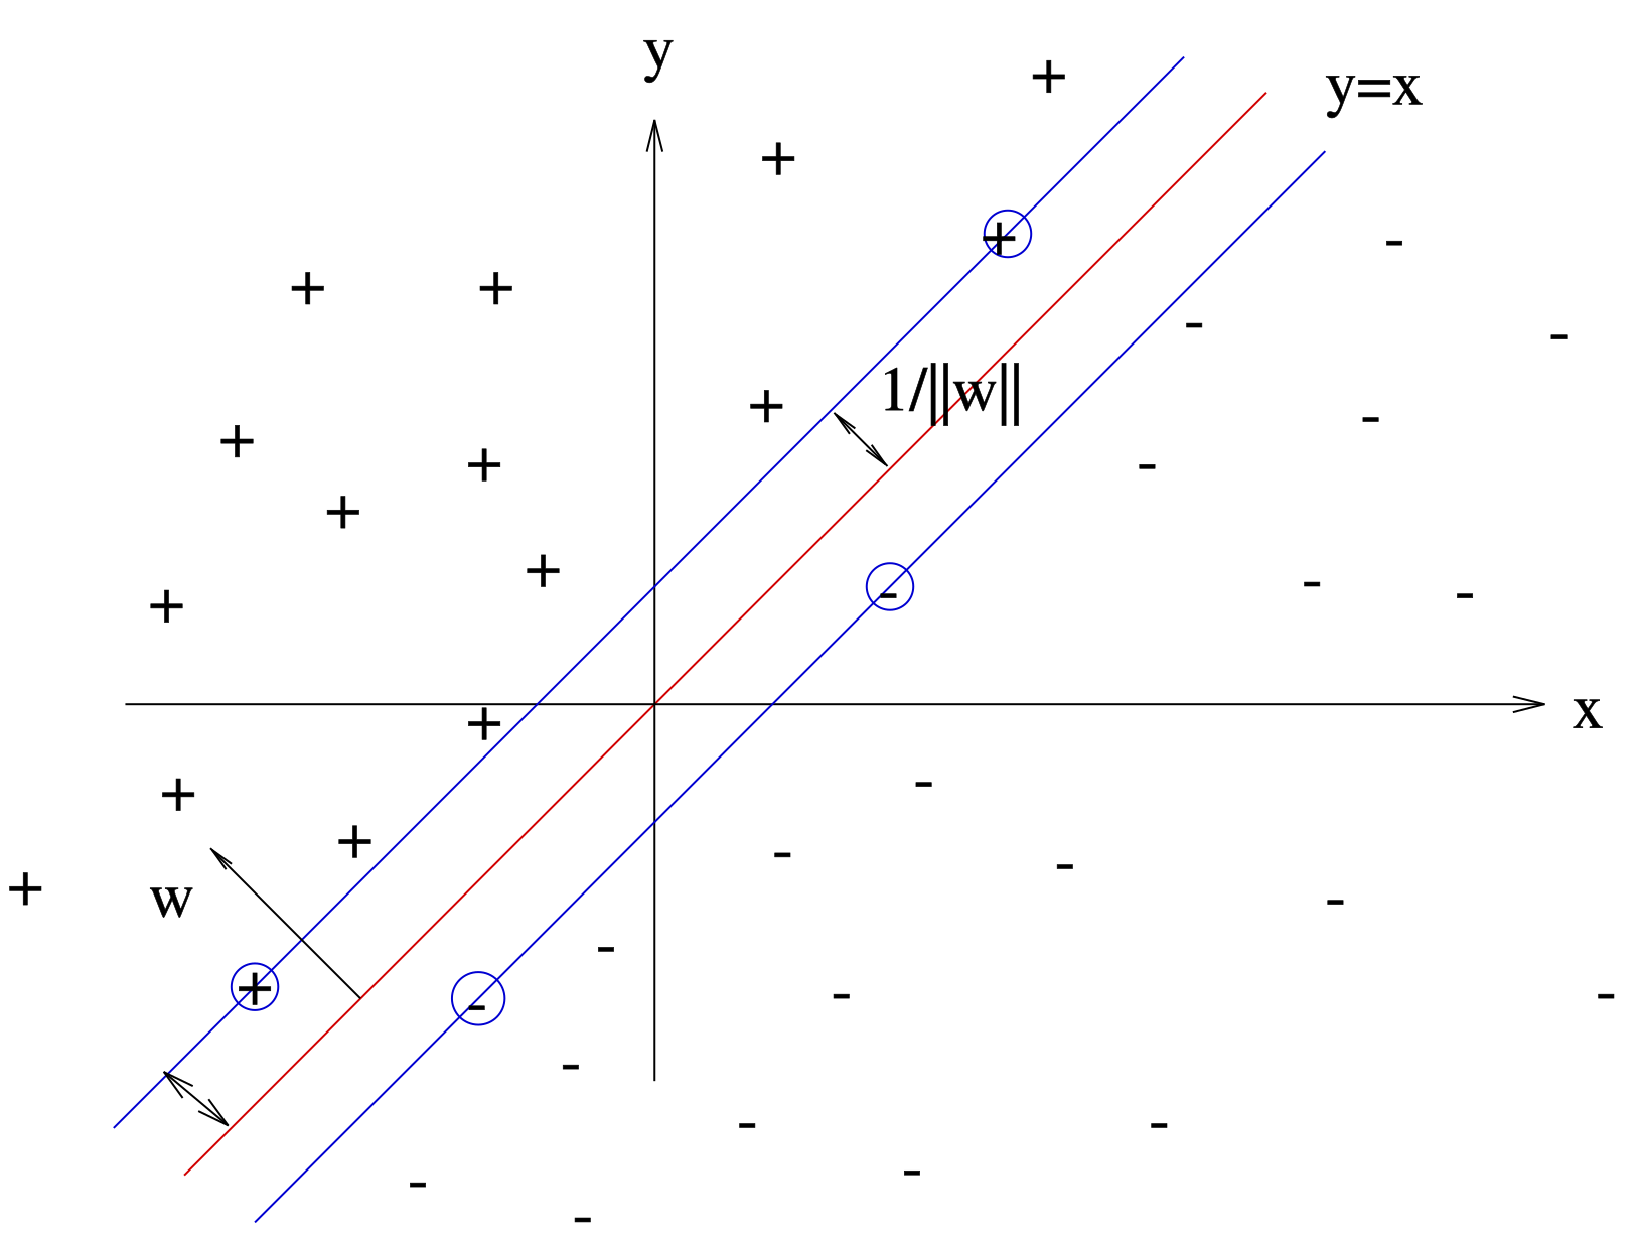
\includegraphics[width=\textwidth]{../images/pipeline/svm_best_boundary.pdf}
        \captionsetup{width=\linewidth}
        \captionsetup{justification=centering}
        \caption{The decision boundary chosen by SVM is based on the maximized distance to the support vectors. Free figure by Sylenius, CC BY-SA 3.0, via Wikimedia Commons.}
        \label{fig:processing_signals_svm_boundary_best}
    \end{subfigure}
    \captionsetup{width=\linewidth}
    \captionsetup{justification=centering}
    \caption{A linearly separable problem with multiple possibilities for decision boundaries.}
    \label{fig:processing_signals_svm_boundary}
\end{figure}


\Gls{svm} assumes that the best decision boundary is the one which maximizes the distance from the \textit{support vectors} to the decision boundary.
These support vectors are the points closest to the decision boundary.
Figure \ref{fig:processing_signals_svm_boundary_best} shows the decision boundary chosen by \gls{svm} based on the maximized distance from the support vectors circled in blue to the decision boundaries shown in red.
In higher dimensionality, this decision boundary becomes a hyperplane which can be described by Equation \ref{eq:processing_signals_svm_decission_boundary} where $\mathbf{W}$ is the weight vector normal to the hyperplane and $b$ is the bias.
The distance from a point $\mathbf{p}$ to this decision boundary can be calculated using Equation \ref{eq:processing_signals_svm_point_distance}.
$||\mathbf{w}||$ denotes the euclidean norm of the weight vector $\mathbf{W}$.

Since we assume a linear separation is possible, we know that for the training samples $\mathbf{x}_i$ with binary class label $y_i$ that Equation \ref{eq:processing_signals_svm_rules} holds.
Since scaling $y_i (\mathbf{w}^T \cdot \mathbf{x}_i + b)$ won't change the position of the hyperplane, it is possible to state that for a certain set $\mathbf{W}$ and $b$ the minimal value is 1 since the result will always be different from zero due to the linear separability assumption and the possibility of scaling.
As such, the distance to the hyperplane at the support vectors can be simplified from $\frac{y_i (\mathbf{w}^T \cdot \mathbf{x}_i + b)}{||\mathbf{w}||}$ to $\frac{1}{||\mathbf{w}||}$.
Maximizing $\frac{1}{||\mathbf{w}||}$ corresponds to minimzining $||\mathbf{w}||$ which is computationally easier and what is done by the \gls{svm} algorithm in an iterative way.


\begin{equation}
    \label{eq:processing_signals_svm_decission_boundary}
    \mathbf{w} \cdot \mathbf{x} + b = 0
\end{equation}

\begin{equation}
    \label{eq:processing_signals_svm_point_distance}
    \text{Distance to point } \mathbf{p} = \frac{\mathbf{w}^T \cdot \mathbf{p} + b}{||\mathbf{w}||}
\end{equation}

\begin{equation}
    \label{eq:processing_signals_svm_rules}
    \mathbf{w}^T \cdot \mathbf{x}_i + b 
    \begin{cases}
          < 0 & \text{if $y_i$ = -1} \\
          > 0 & \text{if $y_i$ = 1}
    \end{cases}
    \Longleftrightarrow y_i (\mathbf{w}^T \cdot \mathbf{x}_i + b) > 0
\end{equation}

With the decision boundary in place, making predictions is trivial.
However, the calculations shown all assume a perfectly linearly separable problem, which is often not the case with real-world data and especially not with \gls{eeg} data.
When making this assumption, the \gls{svm} approach is reffered to as \textit{hard margin} \gls{svm} classification.
To allow for classifying in non-linearly separable problems, \textit{soft margin} \gls{svm} classification has to be used.
Soft margin \gls{svm} classification assumes the samples that stop the linear separation from being possible are noise and can be ignored.
Mathematically this is done by changing the minimum condition from $y_i (\mathbf{w}^T \cdot \mathbf{x}_i + b) = 1$ to $y_i (\mathbf{w}^T \cdot \mathbf{x}_i + b) = 1 - \xi_i$.
$\xi_i$ is called the slack variable and \citet{svm_explained} explains in greater detail how it can be controlled by the hyperparameter $C$, which makes a tradeoff between the maximizing the margin and the number of misclassification on the training data.

Whilst the slack variable allows non-linearly separable problems to be learned by \gls{svm}, it assumes that the classification errors it makes are noise in the data.
As such, it only works well for data that is \textit{almost} linearly separable.
However, \gls{svm} has a clever mechanism for reducing non-linear problems to (almost) linear problems.
By finding a higher dimensional representation of the data, \gls{svm} can reduce a non-linear problem to a linear one.
This is known as the \textit{kernel trick} and an intuitive example is shown in Figure \ref{fig:processing_signals_svm_kernel}.
The specific transformation done in this figure is from 2D to 3D with the kernel function shown in Equation \ref{eq:processing_signals_svm_kernel_function}.
In practice, much more complex kernels are often used, with the most common ones being the linear kernel, the polynomial kernel and the \gls{rbf} kernel.
From these, the \gls{rbf} kernel is the most notable as its feature space has an infinite number of dimensions \citep{ml_book}.
Equation \ref{eq:processing_signals_svm_rbf} shows the \gls{rbf} kernel function.
By tuning the hyperparameter $\sigma$, the smoothness of the decision boundary in the original space can be controlled.

\begin{equation}
    \label{eq:processing_signals_svm_kernel_function}
    \Phi ((x_1, x_2)) = (x_1, x_2, x_1^2 + x_2^2)
\end{equation}

\begin{equation}
    \label{eq:processing_signals_svm_rbf}
    \Phi ((\mathbf{x}, \mathbf{x}')) = \exp(- \frac{|| \mathbf{x} - \mathbf{x}' ||^2}{2 \sigma^2} )
\end{equation}

\begin{figure}[t]
    \centering
    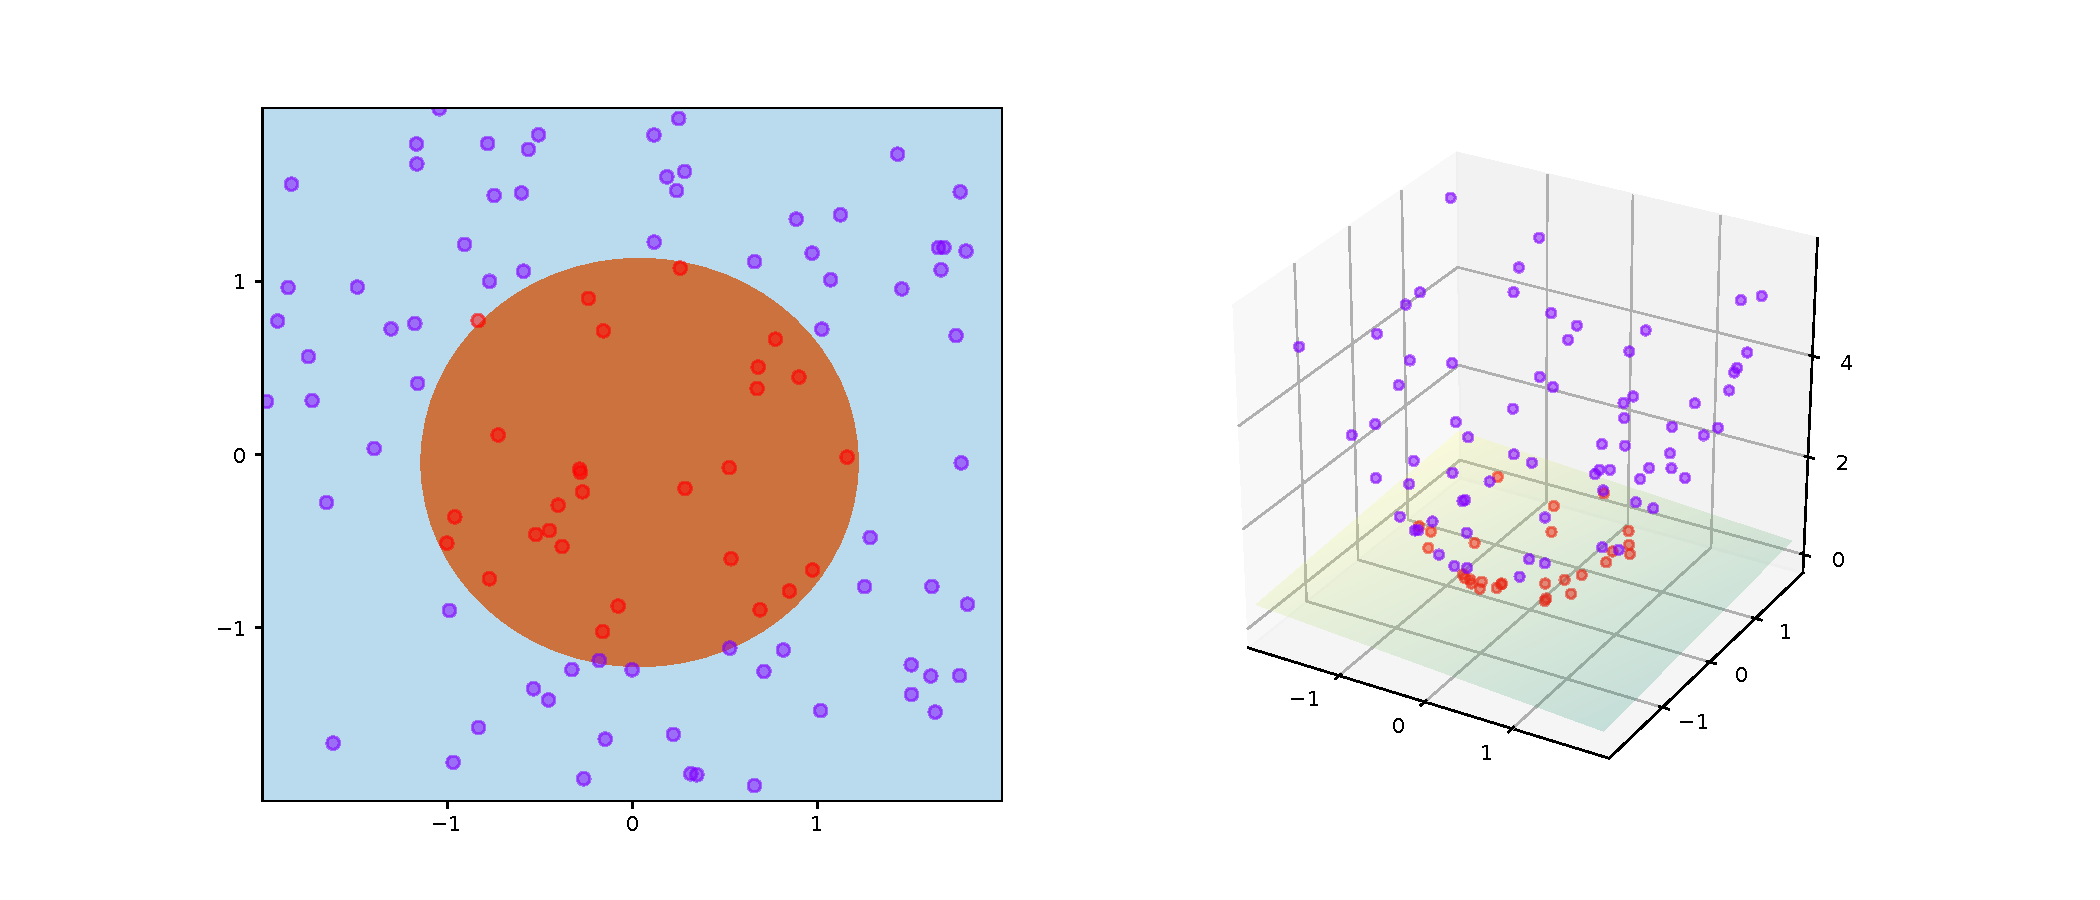
\includegraphics[width=\linewidth]{../images/pipeline/svm_kernel_trick.pdf}
    \captionsetup{width=0.8\linewidth}
    \captionsetup{justification=centering}
    \caption{An intuitive example of SVM's kernel trick where a 2D non-linearly separable problem is transformed into a 3D problem where it is linearly separable. Free to use Figure by Shiyu Ji, CC BY-SA 4.0, via Wikimedia Commons.}
    \label{fig:processing_signals_svm_kernel}
\end{figure}

% | | | | | | | | | | | | |

\subsubsection{Random forest (RF)}
\label{subsubsec:processing_signals_ml_and_dl_ml_classifiers_rf}

To understand the \gls{rf} classifier, decision trees, bootstrapping, aggregation and ensemble learning should first be understood.
Decision trees are a type of classifier that learns how to best split the training data based on certain feature value comparisons.
For example, in a dataset of healthy patients and patients with lung cancer, it might be found that the best first split to make for dividing the data into two most discriminative sets is splitting on whether the subject is younger or older than 60. 
As subsequent splits happen, a tree-like structure is made where every split has a rule, a \textit{decission} and where steps in a particular direction are called branches.
The branches eventually lead to a collection of training data each from the same class.
At this point, further splitting of this branch stops and this last part is called a leaf.
When predicting using the decision tree, each subsequent condition is checked and the tree is decent in the right direction.
When reaching a leaf, the model returns the class label that is most dominant among the training samples in that leaf.
When no additional restrictions are in place, a decision tree can be made that is so big and precise that all training samples are classified correctly, assuming no two training samples are identical but from another class. 
Since this is a clear sign of overfitting, common methods for limiting this behaviour include having a fixed maximum depth (amount of consecutive splits), a minimal amount of samples needed to perform an additional split and more.
The criteria used to determine what split to make is dependent on the implementation, \citet{dec_trees_compared} compares to the most important ones: ID3, C4.5, and CART.

Decision trees on their own are often limited in performance when applied to a complex dataset.
\Gls{rf} works by combining many different decision trees to form a forest, where each decision tree is trained using a bootstrapped version of the training data and an often limited random subselection of features.
Bootstrapping is the simple technique of building a new dataset based on randomly picking examples with replacements from the original training set.
This results in distinct trees, as each tree had different training sets and different features to work with.
In essence, a complex problem is divided into many simplified ones.
having 100 to 2000 decision trees in a random forest is not uncommon.
To decide the final classification, each decision tree's output is collected through a process called aggregation where a majority vote or other technique can be used to determine the final individual classification output of the \gls{rf}.
As \gls{rf} uses both bootstrapping and aggregation, it is often called a \textit{bagging} method.
Since it uses many weaker models to create a strong model, it is often called an \textit{ensemble} method.




% - - - - - - - - - -
% Common DL classifiers
% - - - - - - - - - -

\subsection{Common one-step DL classifier layers}
\label{subsec:processing_signals_ml_and_dl_dl_classifiers}





\Glsfirst{dl} is a subset of \gls{ml} that can be described as any \glsfirst{ann} model that has at least three layers.
\Gls{ann}, often simply reffered to as \gls{nn}, are named after the biological neural network present in the brain and in part discussed in Section \ref{sec:biomedical_signals_biosignals_in_human}.
Where it was discussed the biological neural network consists of many connected neurons that can activate each other in varying strengths based on the number of neurotransmitters released, an \gls{ann} consists of neurons connected through edges which have a learnable weight associated that specifies how much one node activates another.
Figure \ref{fig:processing_signals_mlp} visualizes one of the most basic \gls{nn} possible, a \gls{mlp} with three layers, the minimum amount to be considered a \gls{dl} model.
As discussed in Section \ref{subsec:processing_signals_ml_and_dl_difference}, \gls{nn} are universal function approximators.
For the \gls{mlp} shown in Figure \ref{fig:processing_signals_mlp}, it is a nested function where each layer is seen as a different function.
As such, this \gls{mlp} can be mathematically written as Equation \ref{eq:nn_math}, where $y$ denotes the scalar returned by the singular output node.
The function of the first two layers, $\mathbf{f}_1$ and $\mathbf{f}_2$, are vector functions as these layers consist of multiple neurons.
This mathematical notation is further detailed by \citet{ml_book}.


\begin{equation}
    \label{eq:nn_math}
    y = f_{NN}(\mathbf{x}) = f_3(\mathbf{f}_2(\mathbf{f}_1(x)))
\end{equation}



Sometimes \gls{dl} networks are reffered to as \textit{deep} or \textit{shallow}, as is the case for the DeepConvNet and ShallowConvNet \gls{cnn} based classificiation models considered for the experiments of this master thesis.
These definitions of shallow and deep \gls{nn} are rather ambiguous as following the provided definition of \gls{dl}, any \gls{nn} with more than three layers is considered a deep one.
Concerning the models used in this master thesis, the difference between a shallow and a deep \gls{nn} is that the latter has a significantly large amount of layers whilst the former doesn't.

A \gls{dl} model is defined by the layers it has, of which there consist many different types, too many to be listed here.
As a result, this section only glosses over the layers of most interest for this master thesis.
A focus is put on the intuitive explanation of the concepts with resources provided if more technical detail is desired.
The \gls{dl} book by \citet{dl_book} and the more general book on \gls{ml} by \citet{ml_book} also provide more insight on these layers.
\Citet{ml_dl_book} provides a more hands-on book where the implementation of \gls{dl} models using Keras is discussed.
For the understanding of the \gls{lstm} architecture, the reader is referred to the work by \citet{staudemeyer_understanding_2019}.
Due to time constraints, it was not feasible to provide a detailed discussion on this layer, as it requires the explanation of some general \gls{rnn} concepts as well, which fall outside the scope of this master thesis.
It is important to know that these layers are created with time series in mind and as such are good at working with time series, which \gls{eeg} is.
Their direct focus on this kind of data is why these layers are used for both the extension to EEGNet proposed by this master thesis.

% | | | | | | | | | | | | |

\subsubsection{Multilayer perceptron (MLP)}
\label{subsubsec:processing_signals_ml_and_dl_dl_classifiers_mlp}

\begin{figure}[t]
    \centering
    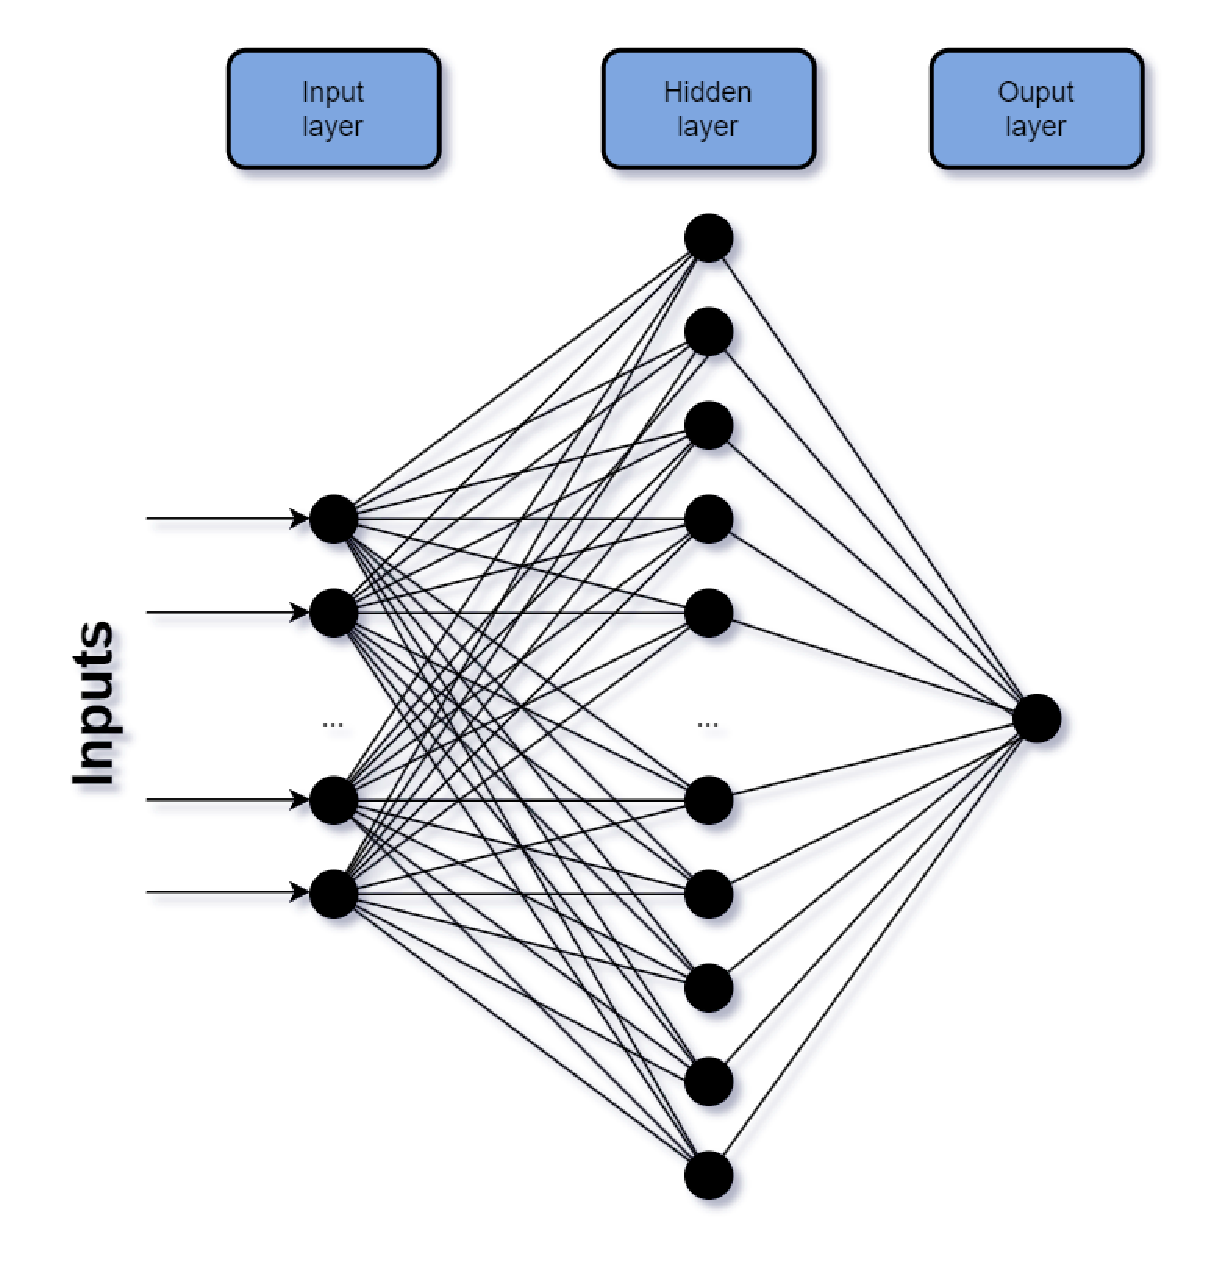
\includegraphics[width=0.5\linewidth]{../images/pipeline/mlp.pdf}
    \captionsetup{width=0.8\linewidth}
    \captionsetup{justification=centering}
    \caption{An example of a three-layer \gls{mlp} with a multidimensional input layer and a one-dimensional output layer. Dots denote neurons and lines denote edges which have an associated weight that can be learned.}
    \label{fig:processing_signals_mlp}
\end{figure}

a \glsfirst{mlp} is one of the simplest types of a \gls{ffnn} and it is often reffered to as a vanilla \gls{nn} \citep{ml_book}.
An \gls{mlp} consists of an input layer, one or more hidden layers and an output layer, all of which can be multidimensional of differing sizes.
Al neurons are fully connected to the neurons in the consecutive layer in a one-directional manner, explaining why they are a type of \gls{ffnn}.
Depending on the activation function used in the output layer, \gls{mlp} can be a function approximator for a classification issue or a regression issue.
For a \gls{mlp} to learn non-linear mappings from input to output, a non-linear activation function has to be used in at least one of its layers.

The architectural design of a \gls{mlp} is conceptually simple.
Despite its simplicity, being a universal function approximator and providing non-linearity through a correct activation function choice, a \gls{mlp} can be very capable.
However, given each neuron is connected to all neurons of the following layer, it is a full-connected \gls{nn} and as such can quickly blow up in the number of trainable parameters when sufficient neurons and layers are used.
Thus, considering the number of edges and neurons present, there are more interesting approaches available.
Whilst none of the models considered in this master thesis made explicit use of a \gls{mlp}, they did make use of a dense layer, which is a fully connected \gls{ff} layer and as such is similar to a singular layer of the \gls{mlp}.





% | | | | | | | | | | | | |

\subsubsection{Activation functions}
\label{subsubsec:processing_signals_ml_and_dl_dl_classifiers_af}

% activation: elu
As discussed, the activation function is what provides the \gls{mlp} with non-linearity.
Intuitively, this is easy to understand as all the neuron has is a sum of weighted inputs and a bias.
None of these operations is non-linear and as such, no non-linear functionality can be learned as is.
When providing the neuron with the activation function, it uses this activation function and passes its sum of weighted inputs to it to obtain the output.
If this activation function is non-linear then the network can learn non-linear mappings.
As such, using non-linear activation functions has almost become a requirement for obtaining capable \gls{nn}.

In theory, any arbitrary function can be used as an activation function and many different activation functions exist.
Choosing the right one can influence the training behaviour of the model a lot.
Whilst not required in theory, most of the time each neuron of a layer uses the same activation function.
This is also denoted in the notation of the \gls{mlp} in Equation \ref{eq:nn_math}.

As described by \citet{dl_book}, the default go to activation function currently is \gls{relu}, the definition for which is given in Equation \ref{eq:relu}.
\gls{relu} was first described by \citet{first_relu}
Whilst this equation looks linear, it is not given the change from a flat line on $0$ for $x<=0$ and a linear function for $x>0$.
\gls{relu} is a simple activation function as it either passes zero or its input value.
As such, using \gls{relu} is computationally efficient, which is one of the reasons it is so popular.
\gls{relu} can also be used as classification function as described by \citet{relu_classi}.

\begin{equation}
    \label{eq:relu}
    ReLU = f(x) = max(0, x)
\end{equation}

However, by far the most famous classification function, especially for multiclass classification is softmax, which is used by all \gls{dl} networks considered in this master thesis and was first introduced by \citet{softmax}.
Softmax provides a value between 0 and 1 for each of the output nodes, the sum of which totals 1.
Strictly taken it is not a probability but rather a certainty metric of the network that happens to total 1.
The network would have to be calibrated on another dataset such that this output indeed represents probabilities \citep{softmcax_calibration}.
The softmax function is given in Equation \ref{eq:softmax}

\begin{equation}
    \label{eq:softmax}
    \text{softmax} = f(x_i) = \frac{e^{x_i}}{\sum_j e^{x_j}}
\end{equation}

Another commonly used activation function is \gls{elu} and is used by most of the \gls{dl} models considered for this master thesis.
It was first proposed by \citet{elu} who argued that despite being slower to calculate than \gls{relu}, it causes faster convergence overall.
It also eliminates the "dead \gls{relu}" problem, where a \gls{relu} activated neuron gets stuck in a position where it always outputs zero and thus is "disabled".
The \gls{elu} function is given in Equation \ref{eq:elu}.
The $\alpha$ parameter is a tunable value between 0 and 1.
It was left at its default of 1 in this master thesis.

\begin{equation}
    \label{eq:elu}
    ELU = f(x) = \begin{cases}
        x  & if x > 0 \\
        \alpha(e^x -1) & otherwise
      \end{cases}
\end{equation}

Many other activation functions exist but are not used in this master thesis.
ShallowConvNet, as proposed by \citet{eeg_model_hbm}, makes use of the self-explanatory square and log activation function.
Activation functions are still an active area of research where gains are still possible, as discussed by \citet{rl_activation_function_compare}.
These gains revolve mainly around having more stable and faster convergence rather than obtaining better accuracy results.



% | | | | | | | | | | | | |

\subsubsection{Convolutional neural networks}
\label{subsubsec:processing_signals_ml_and_dl_dl_classifiers_cnn}

\begin{figure}[t]
    \centering
    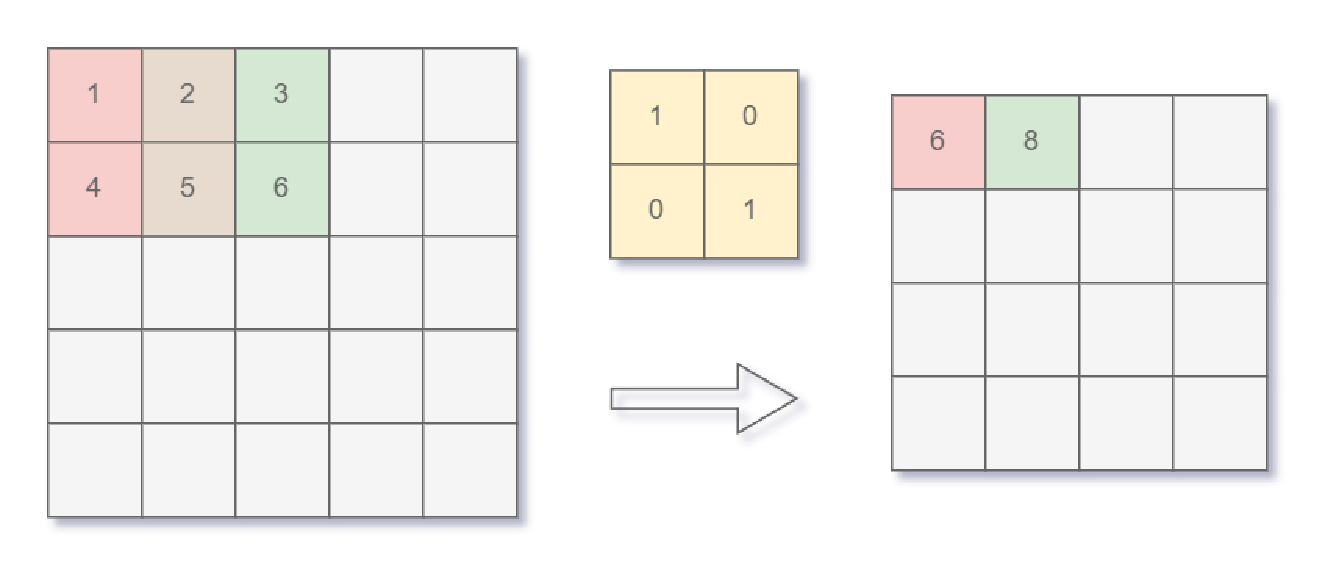
\includegraphics[width=\linewidth]{../images/pipeline/cnn.pdf}
    \captionsetup{width=0.8\linewidth}
    \captionsetup{justification=centering}
    \caption{Visualisation of a convolutional layer.}
    \label{fig:processing_signals_cnn}
\end{figure}


\Gls{cnn} are a type of \gls{nn} consisting of multiple consecutive convolutional layers often having intermediate pooling layers.
A convolution using a 2x2 kernel and stride 1 working over a 2D input is shown in figure \ref{fig:processing_signals_cnn}.
The idea of a convolutional layer is as follows.
For the specified amount of output channels $n$, $n$ different kernels of a specified kernel size are made.
Each of these kernels has trainable parameters which represent the values to use for the convolution.
The kernel passes over the input in a left to right, top to bottom order, stepping by a step size that can be configured as the stride.
On each step, the convolution is calculated and a singular value is placed on the appropriate location of the output.
Taking the convolution of a kernel over the input consists of multiplying the overlapped values and taking the sum.
When no padding is used, as is the case for the example in Figure \ref{fig:processing_signals_cnn}, downsizing occurs due to the kernel reaching the border of the input space.
This reduction corresponds to the size of the kernel in the corresponding orientation minus 1.
Thus for Figure \ref{fig:processing_signals_cnn}, both horizontal and vertical dimensions are reduced by 1.
Settings exist to apply padding, which adds zeros or some other values around the image such that the output dimensions are equal to the input.

It is important to stress that the same kernel weights are used for processing the whole input.
This makes convolutional approaches an interesting approach, as the amount of trainable parameters is limited and it has been shown that convolution layers are excellent at extracting spatially correlated features \citep{cnn_explained}.
When considering the 2D matrix shown in Figure \ref{fig:processing_signals_cnn} as an \gls{eeg} signal, using a kernel of height 1, a 1D convolution is done over the \gls{eeg} signals, without modifying the channels dimension.
This is done by many of the models considered in this master thesis.
The convolutional approach is further described in detail by \citet{cnn_explained}.
When using convolutional networks on a timeseries, it can detect local patterns and as discussed in Section \ref{subsec:offline_bci_system_one_step_dl_eegnet} it can even learn frequency filters.

Besides a convolutional layer, a pooling layer is often used right after a convolutional layer.
Pooling layers are made to reduce the dimensions of their input.
As such, a pooling layer could be seen as a convolutional layer but where the kernel used a predefined fixed function that doesn't learn or adapt itself.
Famous examples of this are max-pooling and mean-pooling.

The proposed models in this master thesis make use of a variant of the conventional layer called depthwise separable convolution and depthwise convolution.
Depthwise separable convolution consists of two steps.
First, a depthwise spatial convolution is performed, this acts on each input channel separately.
Afterwards, a pointwise convolution is performed, this merges the resulting output channels.
These variants are mostly used due to the speed increase they offer, as their outputs can also be achieved by regular multiple regular convolutional steps.
These extension of \gls{cnn} are further discussed by \citet{lu_optimizing_2022} who also discuss further computational optimisations.

% | | | | | | | | | | | | |

\subsubsection{Dropout and batch normalization}
\label{subsubsec:processing_signals_ml_and_dl_dl_classifiers_drop}

Dropout is a layer most commonly used to combat overfitting.
A dropout layer disables random neurons of its input by setting them to zero.
This is done at a given probability.
By doing so, you are forcing neurons to learn from many different neurons, as relying on one neuron for its output will degrade its performance when this neuron is turned off due to the dropout functionality.
Intuitively, this incentivizes neurons to consider the input of more neurons and as such has proven to significantly help in reducing overfitting.
A more detailed explanation as to why this is, is provided by \citet{dropout}.

Batch normalization is a normalization layer.
It collects a batch of samples, determines the mean and standard deviation and provides the normalized samples as output by having them subtracted by the mean and then divided by the standard deviation.
In doing so the values have a zero mean and unit variance.
This helps combat the internal covariate shift problem which is further discussed by \citet{ioffe_batch_2015}.

% ---------------------------------------------- 
% EVALUATING AND USING
% ---------------------------------------------- 
\section{Evaluating the performance of the pipeline}
\label{sec:processing_signals_evaluating_and_using}

Section \ref{subsec:bci_opportunities_obstacles_lack_of_testing} discussed how a lack of standardized methods for both evaluation and reporting in \gls{bc} systems and \glspl{bci} in particular is one of many open issues.
As discussed, the main problem resides in evaluation strategies made for testing specific parts of the \gls{bci} system, such as the classification pipeline, not representing the final performance of the complete system.
However, due to the complexity of proposing a complete \gls{bci} system and performing an in-depth user study of that complete system, it is not feasible for every paper on \gls{bci} related research, including this master thesis, to do such extensive testing on a complete system.

For this reason, it was proposed in section \ref{subsec:bci_opportunities_obstacles_lack_of_testing} that the proposal of a complete \gls{bci} system should happen over at least four distinct papers, each focusing on a specific part.
As discussed, the contents of this master thesis relate most to the second of those four, where classification pipelines are compared and proposed.
As such, most of the evaluation metrics revolve around general \gls{ml} metrics derived from the \gls{cm} on either validation and/or test set.
However, as further discussed by \citet{ml_underspec}, it should be noted that these metrics don't include certain deployment factors and are most often an overestimation of real-world performance.
Besides these general \gls{ml} metrics, some metrics mostly used in testing the performance of medical \gls{ml} can be insightful for evaluating the risks associated with misclassification by the pipeline.
The remainder of this section discusses these topics in more detail.

% | | | | | | | | | | | | |

\subsubsection{The train, validation and test set split}
\label{subsubsec:processing_signals_evaluating_and_using_evaluation_valtest}

To test the performance of a classification pipeline, it is important that testing happens on data that was not used for training.
Intuitively, this has to be done as asking the classifier to classify a sample it has already seen the label for during training, is not going to give any indication of the real-world performance of the algorithm.
A simple 1-nearest neighbour algorithm would score perfectly in such a case and more complex algorithms would be incentivised to overfit to the data rather than learning the problem.

Most commonly, a complete dataset is split into three distinct sets: a training set, a validation set and a test set.
The difference between this validation and test set is their intended use.
For deciding the right parameters of a model, having some data that was not used for training, allows for testing which parameters are performing better.
The validation set is made for these kinds of assessments.
However, extensive use of the validation set will degrade the effectiveness of this set.
Given enough variations of a model, one is bound to perform well on this validation, even if it doesn't learn anything or it is a completely random one.
As such, another set, the test set, is needed for one \textit{final} performance assessment of the model.
It is important to stress that this test set should only be used once for this final assessment as further changes after obtaining an initial test score to improve this test score results in the test set becoming a validation set.
In medical research, a 7:1:2 ratio for training, validation and test split is relatively common \citep{attia}.
However, this is heavily dependent on the amount of data available and the problem at hand.

One issue with splitting the data into a train, validation and test set is that the obtained split is not representative of the data it is taken from or that it suffers from \textit{data leakage}.
Depending on the dataset, it can be a complex task to combat this.
First, samples should be sampled randomly such that each sample has an equal chance of being selected.
Second, the sampling should happen in a stratified manner such that the distribution of classes or other attributes present in the data is respected.
This will reduce the risk that a certain set contains an unreasonably high or low amount of samples from a certain class or attribute.
Take for example a test set for the \gls{mi} \gls{eeg} data where due to unfortunate random sampling the test set consists of only healthy subjects (attribute) and mostly samples from a certain \gls{mi} task (class) whilst the original dataset was balanced across all classes and had stroke patients included as well.
A stratified approach based on the class label and health status of the subject eliminates such a scenario from happening.
Third, no data leakage should happen, which requires taking into consideration certain groupings present in the data.
Data leakage occurs when the training data contains information that directly helps in classifying samples from the validation or test split that is not present for a true unseen sample.
For example, in a 3D medical lung imaging setting for classifying cancerous patients, having images or slices from the same patient in both the training and validation/test set is a common example of data leakage.
Even though the training set does not contain that specific slice or image, it contains closely related data that would not be present for a true unseen sample in real-world applications.
Grouped splits can solve this issue by ensuring all data of a subject is in the same group.
However, when data is limited, ensuring all three of these things can be challenging or even impossible.
Take for example data where all samples of a certain class are also from the same group, making it impossible to satisfy both the grouped or stratified conditions discussed.


% | | | | | | | | | | | | |

\subsubsection{K-fold cross validation}
\label{subsubsec:processing_signals_evaluating_and_using_evaluation_kfold}


Rather than taking a fixed train and validation set, using k-fold \gls{cv} can provide better results.
The intuitive idea behind K-fold \gls{cv} is simple.
Rather than making a train/validation/test split, a train/test split is made using the same reasoning.
This training data is then further divided into K folds, with five to ten being relatively common depending on the number of training samples available. 
The classification pipeline is then trained K times on K-1 of these folds.
The fold that is not used for training, is used as a validation set and this set differs in each of the K training steps.
This results in K different scorings for the validation set and thus allows for determining variance as well.
It should be noted that the folds created have to use the same strategy as a fixed validation split to ensure each split is representative of the data without data leakage.
The algorithm behind K-fold \gls{cv} is given as pseudocode in Algorithm \ref{alg:processing_signals_kfold}.
One major drawback of using K-fold \gls{cv} is that it requires training the classification pipeline K times.
Considering some pipelines can take hours, days or even weeks to train, K-fold \gls{cv} is not always feasible.

\begin{algorithm}
    \caption{K-fold cross-validation}
    \label{alg:processing_signals_kfold}
    \begin{algorithmic}
        \State Divide training data in $K$ folds \Comment{Respecting a certain splitting strategy}
        \State $\text{val\_scores} \gets []$ \Comment{Initialize list of validation scores}
        \For{fold $k_i$ in $K$ folds}
            \State Train model on $K \setminus k_i$
            \State $\text{val\_scores} \gets \text{val\_scores} + $ metrics for validation set $k_i$ 
        \EndFor
        \State process $\text{val\_scores}$ as desired
    \end{algorithmic}
\end{algorithm}


% | | | | | | | | | | | | |

\subsubsection{The confusion matrix and its derived scores}
\label{subsubsec:processing_signals_evaluating_and_using_evaluation_cm} 

\begin{figure}[t]
    \centering
    \begin{subfigure}{0.45\textwidth}
        \centering
        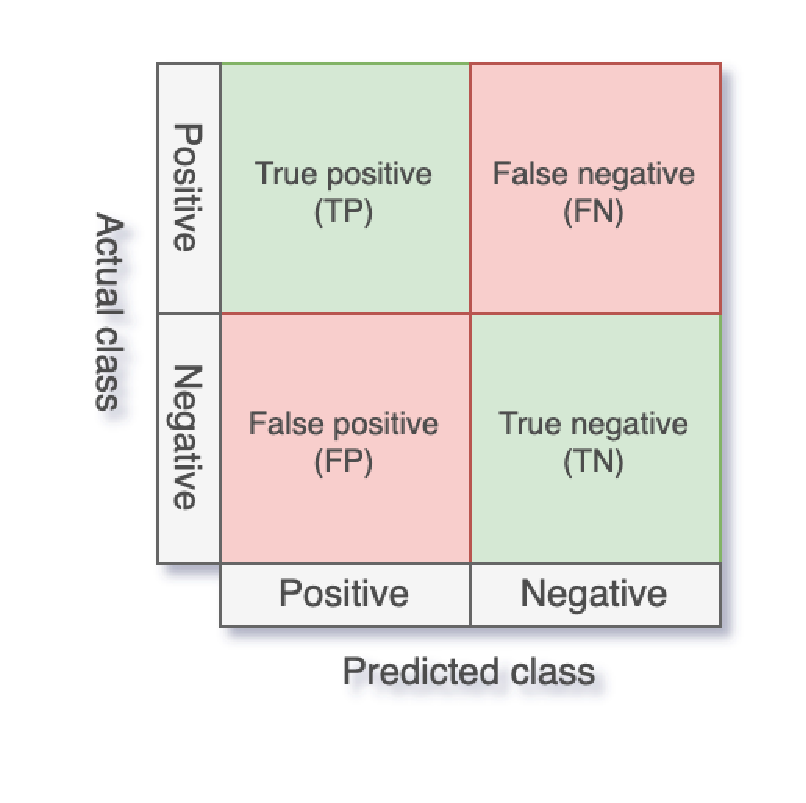
\includegraphics[width=\textwidth]{../images/pipeline/cm_binary.pdf}
        \captionsetup{width=\linewidth}
        \captionsetup{justification=centering}
        \caption{Confusion matrix for a universal binary classification problem.}
        \label{fig:processing_signals_cm_binary}
    \end{subfigure}
    \hfill
    \begin{subfigure}{0.45\textwidth}
        \centering
        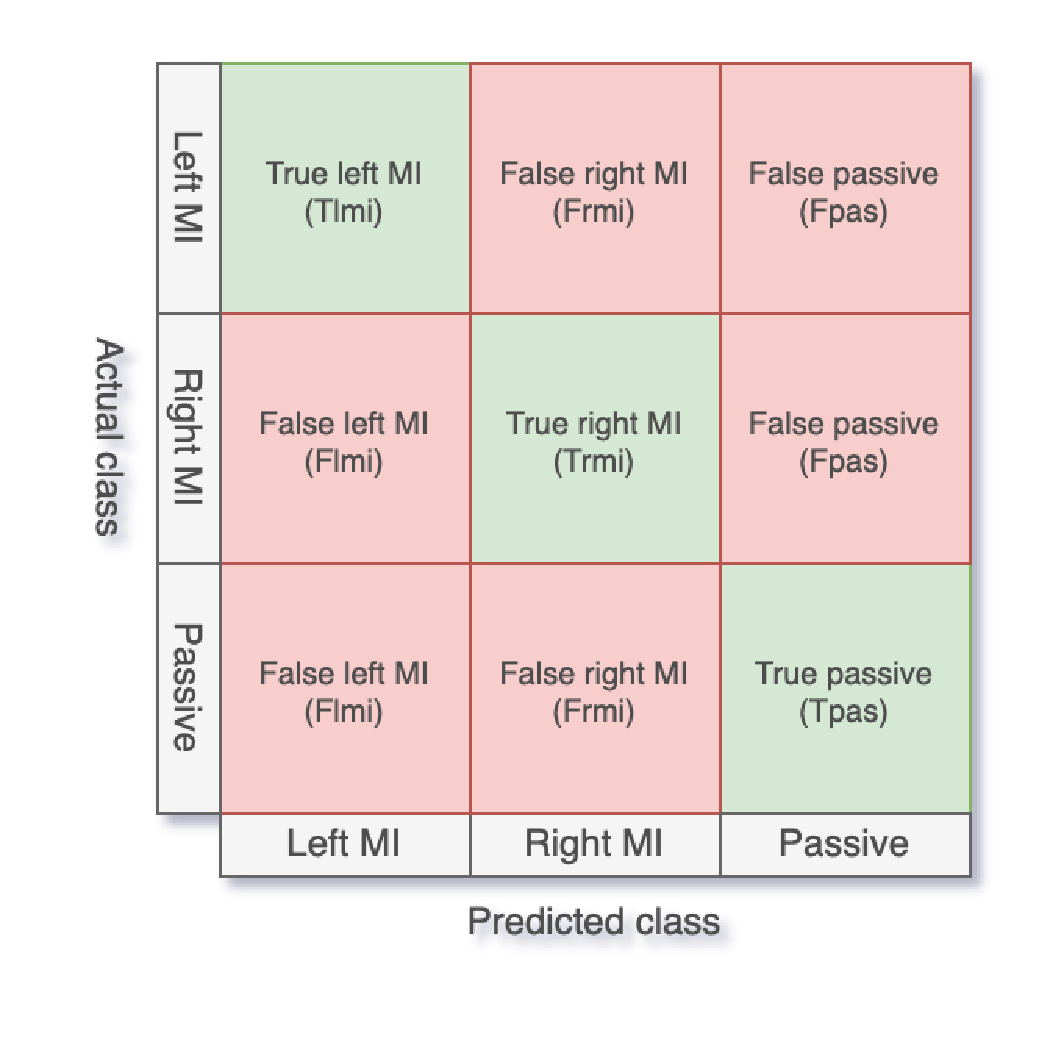
\includegraphics[width=\textwidth]{../images/pipeline/cm_three_class.pdf}
        \captionsetup{width=\linewidth}
        \captionsetup{justification=centering}
        \caption{Confusion matrix for a three-class \gls{mi} classification problem.}
        \label{fig:processing_signals_cm_three}
    \end{subfigure}
    \captionsetup{width=\linewidth}
    \captionsetup{justification=centering}
    \caption{Design of a binary and three-class confusion matrix.}
    \label{fig:processing_signals_cm}
\end{figure}

The \gls{cm} is a simple but powerful tool for visualising the predictions made by a classification pipeline.
The structure of a \gls{cm} for both a universal binary classification problem and a three-class \gls{mi} classification problem is shown in Figure \ref{fig:processing_signals_cm}.
Many of the metrics used for evaluating the performance of a classification pipeline are derived from this \gls{cm}.
Take for example the most commonly used classification accuracy metric, it can be derived by equation \ref{eq:processing_signals_accuracy}.

\begin{equation}
    \begin{aligned} 
        \text{Binary accuracy} &= \frac{TP + TN}{TP + FN + FP + TN} \\\\
        \text{Three-class accuracy} &= \frac{\sum\limits_{x \in \text{classes}} T_x}{\sum\limits_{x \in \text{classes}} F_x}
    \end{aligned}
    \label{eq:processing_signals_accuracy}
\end{equation}

However, reporting on accuracy alone is often not enough as it is also interesting to know what the per-class performance is.
For this, sensitivity (also known as recall) and specificity are also commonly reported.
Their binary formulea are given in Equation \ref{eq:processing_signals_sensitivity} and \ref{eq:processing_signals_specificity} respectively.
Sensitivity gives information on the fraction of true samples being predicted as true whilst specificity provides the fraction of false samples being predicted as false.
For a \gls{cm} where more classes are present, the specificity and sensitivity per class can be calculated similarly.

\begin{equation} % recall
    \text{Binary sensitivity} = \frac{TP}{TP + FN}
    \label{eq:processing_signals_sensitivity}
\end{equation}

\begin{equation}
    \text{Binary specificity} = \frac{TN}{TN + FP}
    \label{eq:processing_signals_specificity}
\end{equation}

Whilst specificity and sensitivity already provide more information, these metrics don't report nicely on unbalanced datasets.
Assume a binary test setting where only 5\% of the samples are of the true class, something that is relatively common for medical conditions such as \gls{af}.
Papers studying the classification of this phenomenon, such as the one by \citet{attia}, will often boast a good specificity and sensitivity, i.e. \citet{attia} reported both to be above 80\%.
However, due to the class imbalance, these metrics are not sufficient on their own or in combination with the classification accuracy.
A mention of the \gls{ppv} and \gls{npv} is also needed.
The binary formulea for which are given in Equation \ref{eq:processing_signals_ppv} and \ref{eq:processing_signals_npv} respectively. 
The \gls{ppv} specifies how many of the samples labelled as true are actually true, the \gls{npv} does the same but for negatives.
Whilst not reported in the previously mentioned paper by \citet{attia}, the \gls{ppv} was found to be under 30\% \citep{ppv_attia}.
In contrast with the high sensitivity and specificity, this would mean that for less than one in three times the model predicted true, the sample was indeed true.
Relating this back to a \gls{bci} system, if the sensitivity and specificity of a risky action are good but the \gls{ppv} is not reported and turns out to be poor due to an imbalance in the testing strategy, the model can not be used in a real-world application as so many unwanted executions of risky actions are not acceptable.
The \gls{ppv} is also referred to as the precision of a model.
The \gls{ppv} and \gls{npv} can also be determined for each class independently in case of a multi-class classification problem.

\begin{equation} % Precision
    \text{PPV} = \frac{TP}{TP + FP}
    \label{eq:processing_signals_ppv}
\end{equation}

\begin{equation}
    \text{NPV} = \frac{TN}{TN + FN}
    \label{eq:processing_signals_npv}
\end{equation}

A final metric that is often reported is the F1 score.
The F1 score is also derived from the idea that sensitivity alone isn't enough for imbalanced data.
To solve this, it provides the harmonic mean of the \gls{ppv} and the sensitivity.
It's binary formula is given in Equation \ref{eq:processing_signals_f1}. 

\begin{equation}
    F1 = 2 * \frac{PPV * \text{sensitivity}}{PPV + \text{sensitivity}}
    \label{eq:processing_signals_f1}
\end{equation}

% | | | | | | | | | | | | |

\subsubsection{The ROC curve and choosing classification thresholds}
\label{subsubsec:processing_signals_evaluating_and_using_evaluation_risk} 

\begin{figure}[t]
    \centering
    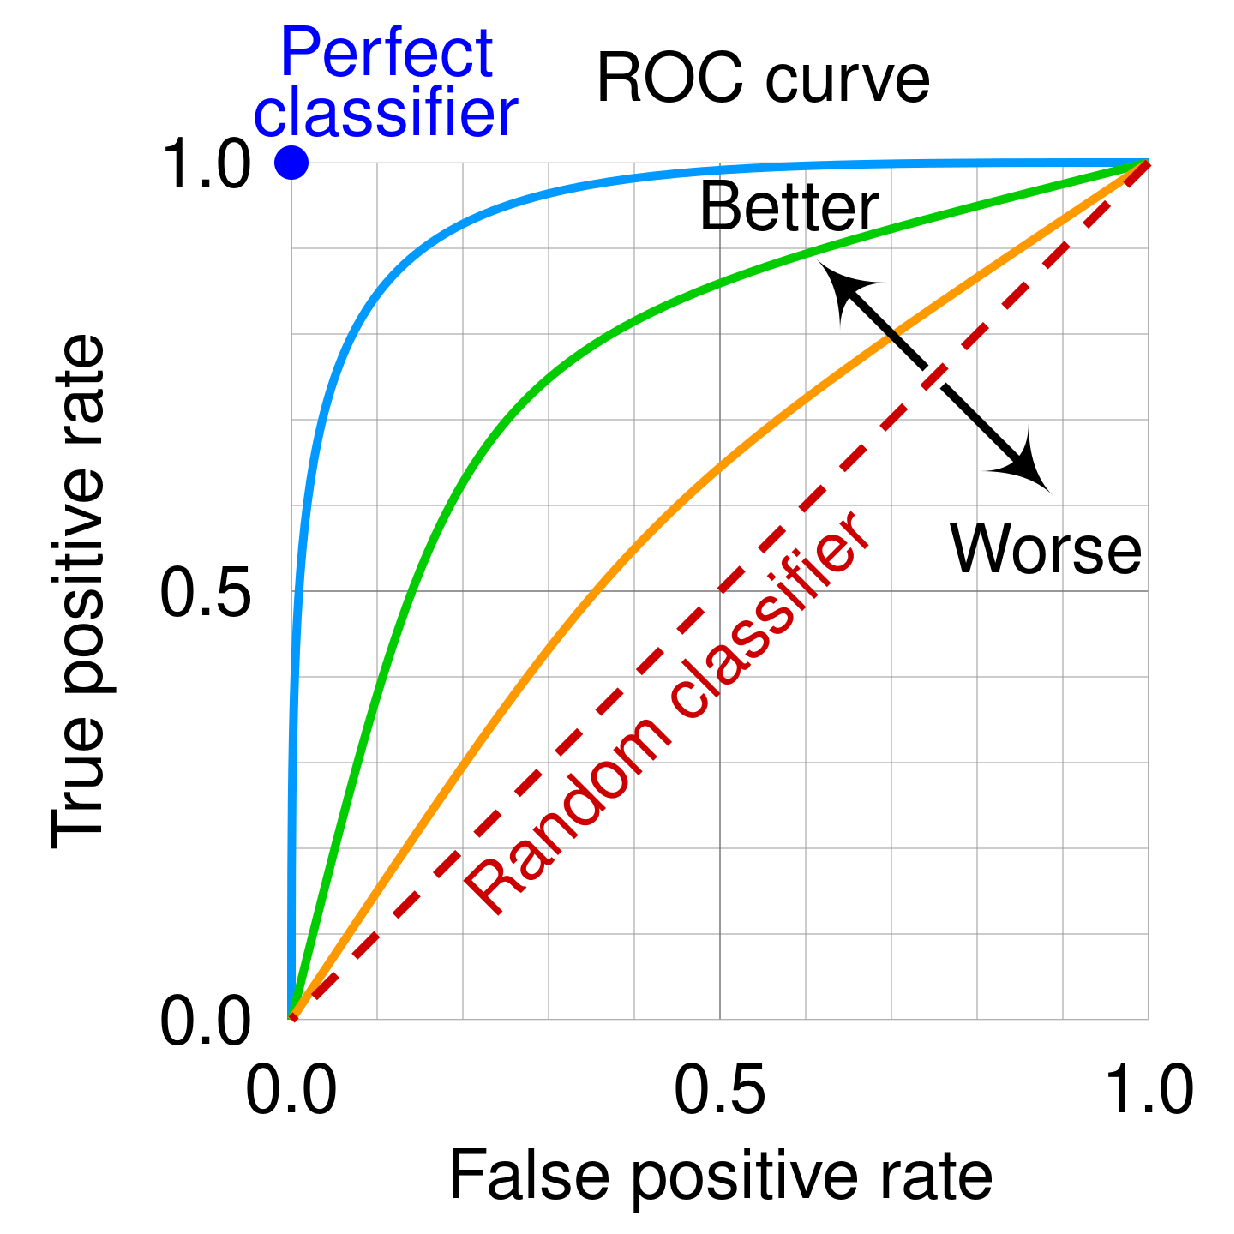
\includegraphics[width=0.6\linewidth]{../images/pipeline/ROC.pdf}
    \captionsetup{width=0.7\linewidth}
    \captionsetup{justification=centering}
    \caption{ROC curve with some arbitrary examples. Free to use figure by cmglee, MartinThoma, CC BY-SA 4.0, via Wikimedia Commons.}
    \label{fig:processing_signals_roc_explained}
\end{figure}

Besides the \gls{cm}, the \gls{roc} is also a powerful tool for visualising the performance of a classification pipeline.
The idea behind the \gls{roc} curve is to visualize the model's performance when making a trade-off between sensitivity (also known as the true positive rate) and the false positive rate (1 - sensitivity).
This trade-off can be controlled by changing the threshold at which a prediction made by the model is considered a prediction of the true label.
By default, this is when the model returns a prediction of 0.5 or higher for the true class, but changing this value can yield more preferred behaviour.
For example, lowering the threshold will make the model classify samples as positive more often, resulting in an equal or higher sensitivity (desired) but also an equal or higher true negative rate (not desired).
Lowering the threshold value does the reverse.
Finding the best balance between both is application specific.
An example of this graph with some examples to demonstrate its working is shown in Figure \ref{fig:processing_signals_roc_explained}.
The \gls{roc} curve is often used to determine the optimal threshold value.
The \gls{auc} is also derived from the \gls{roc} curve as a common evaluation metric.

% ---------------------------------------------- 
% CONCLUSIONS OF CHAPTER
% ---------------------------------------------- 
\section{Chapter conclusions}
\label{sec:processing_signals_summary}

This chapter revolved around the discussion of a general pipeline for classifying brain signals.
By discussing five different components and providing some examples of the techniques available within each component, all required insights for understanding the seven proposed classification pipelines in the next chapter should be provided.
A discussion on which evaluation metrics are recommended to report was also given.
This included a discussion on both general \gls{ml} metrics and metrics more tailored towards the biomedical field where risk factors are more important than overall accuracy results.
It was reasoned that this is also the case for \gls{bci} systems, especially those that can execute risky actions.
Unfortunately, due to time constraints, it was not feasible to report on the \gls{lstm} layers, although the references provided explain this layer in great detail.